\documentclass[twocolumn]{aastex63}

\usepackage{amsmath}
\usepackage{empheq}
\usepackage{mathrsfs}
\usepackage{textcomp}
%\usepackage{enumitem}   
\usepackage{gensymb}
\usepackage{hyperref}
\usepackage{graphicx}
\usepackage[caption=false]{subfig}
\usepackage{multirow}
\usepackage{longtable}
\usepackage{booktabs} % To thicken table lines
\usepackage{CJK}
\bibliographystyle{aasjournal}
\hypersetup{colorlinks, linkcolor={blue}, citecolor={blue}, urlcolor={blue}} 

%\usepackage{lineno}
% \linenumbers

\newcommand{\vdag}{(v)^\dagger}
\newcommand\aastex{AAS\TeX}
\newcommand\latex{La\TeX}

%%%%%%%%%%%%%%%%%%%%%%%%%%%%%%%%%%%%%%%%%%%%%%%%%%%%%%%%%%%%%%%%%%%%%%%%%%%%%%%%
%%
%% The following section defines new commands for comments from co-authors
%%
\definecolor{DarkOrange}{RGB}{204, 85, 0}
\definecolor{LincolnGreen}{RGB}{17, 102, 0}
\def\ion#1#2{#1$\;${\footnotesize\rm{#2}}\relax}

\newcommand{\yy}[1]{{\color{red} yy: {#1}}}
\newcommand{\kde}[1]{{\color{DarkOrange} kde: {#1}}}
\newcommand{\todo}[1]{{\color{magenta} to-do: {#1}}}

\newcommand{\rztf}{$r_\mathrm{ZTF}$}
\newcommand{\gztf}{$g_\mathrm{ZTF}$}
\newcommand{\tfl}{$t_\mathrm{fl}$}
\newcommand{\trise}{$t_\mathrm{rise}$}
\newcommand{\tbmax}{$t_{B,\mathrm{max}}$}
\newcommand{\package}[1]{\textsc{#1}}
%%
%%%%%%%%%%%%%%%%%%%%%%%%%%%%%%%%%%%%%%%%%%%%%%%%%%%%%%%%%%%%%%%%%%%%%%%%%%%%%%%%

%% Reintroduced the \received and \accepted commands from AASTeX v5.2
%\received{\today}
% \revised{January 10, 2019}
% \accepted{\today}
%% Command to document which AAS Journal the manuscript was submitted to.
%% Adds "Submitted to " the argument.

%\submitjournal{ApJ}

%%%%%%%%%%%%%%%%%%%%%%%%%%%%%%%%%%%%%%%%%%%%%%%%%%%%%%%%%%%%%%%%%%%%%%%%%%%%%%%%
%%
%% The following section outlines numerous optional output that
%% can be displayed in the front matter or as running meta-data.
%%
%% If you wish, you may supply running head information, although
%% this information may be modified by the editorial offices.
\shorttitle{AT2019dge: transitional Type Ibn SN?}
\shortauthors{Yao et al.}

%%
%% You can add a light gray and diagonal water-mark to the first page 
%% with this command:
\watermark{DRAFT}
%% where "text", e.g. DRAFT, is the text to appear.  If the text is 
%% long you can control the water-mark size with:
%% \setwatermarkfontsize{dimension}
%% where dimension is any recognized LaTeX dimension, e.g. pt, in, etc.
%%
%%%%%%%%%%%%%%%%%%%%%%%%%%%%%%%%%%%%%%%%%%%%%%%%%%%%%%%%%%%%%%%%%%%%%%%%%%%%%%%%

%% This is the end of the preamble.  Indicate the beginning of the
%% manuscript itself with \begin{document}.

\begin{document}
\pagenumbering{arabic}
\begin{CJK*}{UTF8}{gbsn}

\title{AT2019dge:}

%\author[0000-0001-6747-8509]{Yuhan Yao (姚雨含)}\email{yyao@astro.caltech.edu}
%\affiliation{Cahill Center for Astrophysics, 
%             California Institute of Technology, 
%             1200 E.~California Boulevard, Pasadena, CA 91125, USA}

%\author{Friends}

% KDE

% Zhihui


\begin{abstract}

We present observations of the hydrogen-deficient optical transient AT2019dge/ZTF18abfcmjw. With 
a rise to maximum light of $\lesssim 3$\,days over two magntiude in $g$ and $r$-bands, AT2019dge is 
the most rapidly-rising subluminous Type I supernova (SN) discovered so far. Spectra obtained shortly 
after discover reveal \ion{He}{II} flash emission, with broad \ion{He}{I} features developed $\sim12$\,d 
after peak luminosity. \todo{more to come.} AT2019dge poses chanllenge for existing models of 
fast-rising SNe.

\end{abstract}

%% Keywords should appear after the \end{abstract} command. 
%% See the online documentation for the full list of available subject
%% keywords and the rules for their use.
\keywords{supernovae: general -- supernovae: individual (AT2019dge/ZTF18abfcmjw) -- surveys}

%% From the front matter, we move on to the body of the paper.
%% Sections are demarcated by \section and \subsection, respectively.
%% Observe the use of the LaTeX \label
%% command after the \subsection to give a symbolic KEY to the
%% subsection for cross-referencing in a \ref command.
%% You can use LaTeX's \ref and \label commands to keep track of
%% cross-references to sections, equations, tables, and figures.
%% That way, if you change the order of any elements, LaTeX will
%% automatically renumber them.
%%
%% We recommend that authors also use the natbib \citep
%% and \citet commands to identify citations.  The citations are
%% tied to the reference list via symbolic KEYs. The KEY corresponds
%% to the KEY in the \bibitem in the reference list below. 

\vspace{1em}

\section{Introduction}
The physical origin of the population of subluminous fast-evolving supernovae (SNe) still remains 
largely elusive. Their light curves have been explained by low ejecta mass ($\lesssim 0.5M_\odot$) 
explosions that produce a small amount ($\lesssim 0.1M_\odot$) of radioactive material 
\citep{Shen2010, Sim2012, Moriya2017, Polin2019}, interaction with an stellar envelop or circumstellar 
material (CSM) (e.g. \citealt{KleiserKasen2018, Piro2015}), or even powered by alternative power 
sources, such as an internal engine (e.g. \citealt{Hotokezaka2017}). See \citet{Kasen2017} for a review.

Today, a growing number of SNe are detected within one or two days of the explosion, opening a new 
window into the relatively unexplored early phase of these events. Here we report observations of the 
rapidly evolving subluminous SN AT2019dge discovered by the Zwicky Transient Facility (ZTF; 
\citealt{Bellm2019b}; 
\citealt{Graham2019}), along with modeling of the bolometric lightcurve and early spectra, and a 
discussion of plausible explosion scenarios of this object.

Calculations in this paper assume a $\Lambda$CDM cosmology with $H_0= 70 \, \rm km \, s^{-1}\, 
Mpc^{-1}$, $\Omega_m = 0.27$ and $\Omega_{\Lambda} = 0.73$ \citep{Komatsu2011}. UT times are 
used throughout the paper. Alongside this paper, we have released our open-source analysis and all of 
the data utilized in this study. These are available online at 
\url{https://github.com/yaoyuhan/AT2019dge}. All spectra and photometry will also be made available 
by the WISeREP repository \citep{Yaron2012}.

\section{Observations} 
\subsection{The Detection}
\begin{figure}[htbp!]
    \centering
    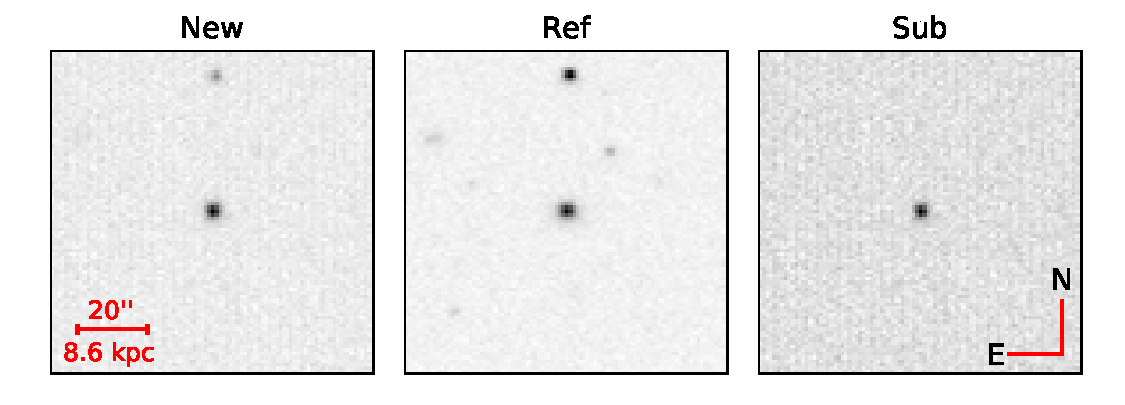
\includegraphics[width=\columnwidth]{figures/detection.pdf}
    \caption{ZTF $g$ band images centered on AT2019dge on Apr 10. From left to right are the new 
    image, the reference image, and the subtraction image. \ \label{fig:detection}}
\end{figure}
\begin{figure*}[htbp!]
	\centering
	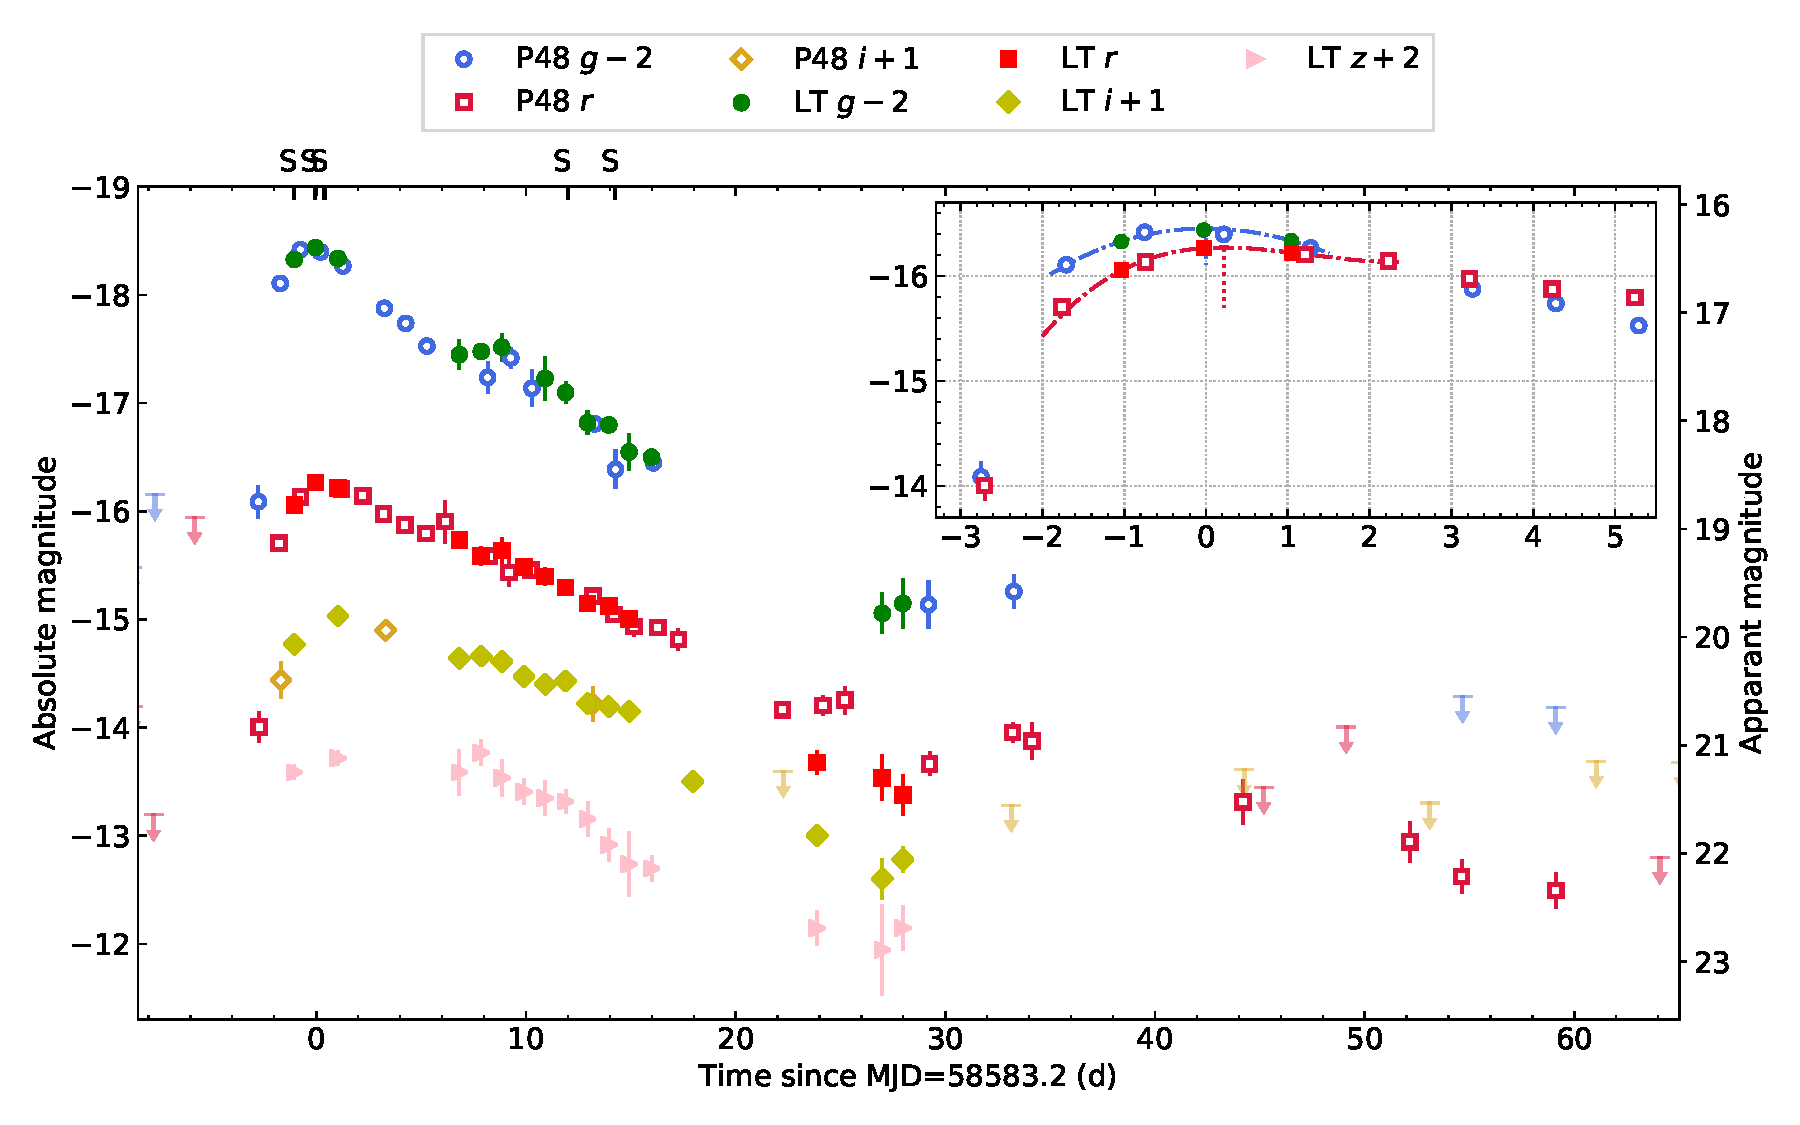
\includegraphics[width=\textwidth]{figures/lightcurve.pdf}
	\caption{Galactic extinction corrected light curve of AT2019dge. The inset shows 
		the light curve zoomed into the region of maximum light. Epochs of spectroscopy are marked with 
		the letter `S' along the upper axis.
		\todo{maybe consider grey-shade the 8 day region since there might be a g band minimum? 
		constrain Rcore?} \label{fig:lightcurve}}
\end{figure*}
% In this section, I report values on Marshal
AT2019dge was first detected by ZTF using the Palomar Oschin Schmidt 48 inch (P48) telescope in a 
one-day cadence experiment. On 2019 April 7 10:18:46 (JD 
$=2458580.9297$), a $g$-band detection at $20.66\pm0.34$ mag and J2000 coordinates $\alpha = 
17^{\mathrm{h}}36^{\mathrm{m}}46.75^{\mathrm{s}}$, $\delta = 
+50^{\mathrm{d}}32^{\mathrm{m}}52.2^{\mathrm{s}}$
%$\alpha = 17^{\mathrm{h}}36^{\mathrm{m}}46.76^{\mathrm{s}}$, $\delta = 
%+50^{\mathrm{d}}32^{\mathrm{m}}52.5^{\mathrm{s}}$ (J2000) 
met the machine-learning thresholds \citep{Mahabal2019} and real-time alerts were generated 
\citep{Patterson2019}. On April 8, the 
transient was flagged by a science program filter on the GROWTH Marshal \citep{Kasliwal2019} that is 
designed to look for fast evolving transients (Ho et al., in prep). 

AT2019dge is consistent with being at the nucleus of a compact galaxy at the redshift of $z=0.0213$ 
(Appendix \ref{app:spec}). Figure~\ref{fig:detection} shows the detection image on April 10. 
 
\subsection{Photometry}

\subsubsection{Optical Photometry} \label{subsubsec:opt_phot}
We perform forced PSF photometry on ZTF difference images following the steps illustrated in 
\citet{Yao2019}. 
%As is mentioned in \citet{Yao2019}, forced photometry provides better constrains on the 
%pre-explosion limits as well as deeper late-time photometry by binning the flux measurements taken 
%at 
%the same night \todo{Is forced photometry the same as binning the flux, or are they separate?  As 
%written implies they are the same -reword? -esp}.
%We fix the position by using the median of all 5$\sigma$ detection coordinates (), which is more 
%accurate than the coordinate of the first detection. 
The sky region of AT2019dge is covered by two ZTF fields with fieldid 763 and 
1799. We exclude all data in field 1799 since the reference image was constructed using images 
obtained between May 25 2018 and July 12 2019, which is after the explosion of the 
transient\footnote{The ZTF name (ZTF18abfcmjw) indicates that the transient was discovered in 2018. 
However, this is due to a candidate detection from negative subtraction (ref minus sci) in 2018 in field 
1799.}.

Since field 763 was included in both the northern sky survey with two epochs (one 
$g\, +$ one $r$) per three nights and the extragalactic high-cadence survey with six epochs (three 
$g\,+$ three $r$) per night\footnote{See \citet{Bellm2019a} for the ZTF experiments design.}, this 
transient are visited muliple times every night. Therefore, single-night flux measurements in the same 
filter are binned (by taking the inverse variance-weighted 
average), which gives a pre-explosion $r$-band limit of 18.95 mag (5$\sigma$ limit computed at the 
expected position of the transient) on April 4 10:36:34. Five-$\sigma$ detections are converted to 
magnitude for further analysis.

Following the discovery of AT2019dge, we obtained follow-up photometry in $griz$ with the optical 
imager (IO:O) on the Liverpool Telescope (LT; \citealt{Steele2004}). LT and P48 photometry are shown 
in Figure~\ref{fig:lightcurve}. Absolute magnitude is determined 
by correcting for the distance modulus and Galactic extinction $E(B-V)=0.022$ estimated by 
\citet{Schlafly2011}, which builds upon \citet{Schlegel1998}. We assume $R_V=3.1$, and adopt
reddening law from \citet{Cardelli1989}. We do not correct for host-galaxy contamination given the 
absence of \ion{Na}{I} D absorption in all spectra at the host redshift. 

We also performed forced photometry on archival PTF/iPTF difference images spanning May 07 2009 to 
June 13 2016\footnote{We followed the procedure described in 
	\url{http://web.ipac.caltech.edu/staff/fmasci/home/miscscience/forcedphot.pdf}}. No historical 
detections was found. 

\subsubsection{Swift Photometry}
 
Space-based observations with the \textit{Neil Gehrels Swift Observatory} (\textit{Swift}; 
\citealt{Gehrels2004}) was triggered on April 9 and April 10. Ultraviolet/Optical Telescope (UVOT; 
\citealt{Roming2005}) data were obtained in the $UVW1$, $UVM2$, $UVW2$, $U$, $B$, and $V$ 
filters. 

UVOT data are reduced using HEAsoft (v6.17) with a $3^{\prime\prime}$ circular aperture. To remove 
host-galaxy contribution at the location of 
the SN, we obtained a final epoch in all broad-band filters on June 23 2019 and measured the 
photometry with the same aperture used for the transient. 

We note that no point sources were detected in the XRT event files with $\rm{SNR}>2$.

\subsubsection{Radio Follow-up}
We observed at high frequency radio bands using the Submillimeter Array (SMA, \citealt{Ho2004}) on 
UT 2019 xx xx under its target-of-opportunity program. The project ID was xxx. Obser


\subsection{Spectroscopy}

We obtained seven optical spectroscopic follow-up of AT2019dge  starting from $-10$\,d to $+53$\,d 
after $r$-band peak using the Rapid Acquisition of Transients (SPRAT; \citealt{Piascik2014}) on the 
Liverpool Telescope (LT), the Double Spectrograph (DBSP) on the 200-inch Hale telescope 
\citep{Oke1982}, and the Low Resolution Imaging Spectrograph (LRIS) on the Keck-I telescope 
\citep{Oke1995}. We present our sequence of spectra in Figure~\ref{fig:spectra}. 

We use the automated LT pipeline reduction and extraction for the LT spectra. LRIS spectra were 
reduced and extracted using \texttt{Lpipe} \citep{Perley2019lpipe}. The DBSP spectrum was reduced 
using a \texttt{PyRAF}-based reduction pipeline \citep{Bellm2016}.

\todo{HST UV Spectroscopy}
G280 grism

70@300nm and an average dispersion of about 1.3 nm per pixel

Since there is no detectable \ion{Na}{I} D lines in any of our spectra and the object is very blue, we 
assume throughout the analysis that the host extinction along the line of sight is negligible.


\section{Basic Properties of the Explosion \\and its Host Galaxy}
\subsection{Light Curve Properties}\label{subsec:lc_properties}

To estimate the epoch of maximum light, we interpolated the $g$- and $r$-band photometry with 
three-order polynomial functions, as is shown in the inset of Figure~\ref{fig:lightcurve}. The time range 
used in the fit is from ${\rm MJD}=58581.2$ to $58585.2$. AT2019dge was found to peak 
at $M_{g, \rm max}=-16.45\pm0.04$ mag on ${\rm MJD}=58583.19$, and $M_{r, \rm 
max}=-16.27\pm0.02$ mag on ${\rm MJD}=58583.39$. Hereafter we use $\Delta t$ to denote time
with respect to the $g$-band maximum light epoch, ${\rm MJD}=58583.2$, and use $t$ to denote time 
from the assumed explosion epoch (MJD = xx measured from Section xx).

\begin{figure}[!htbp] 
	\centering
	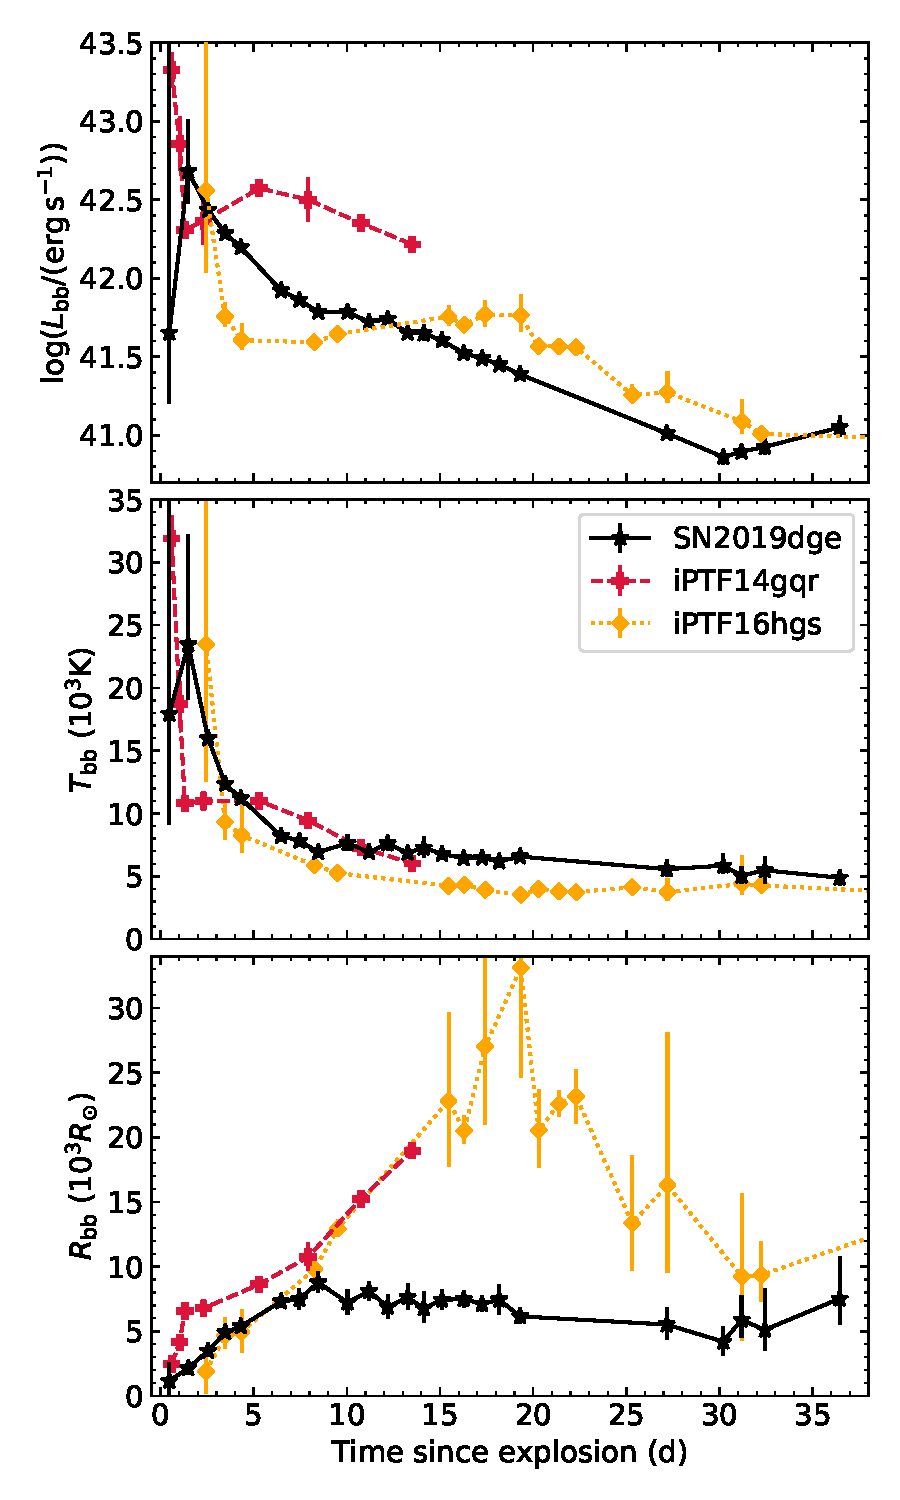
\includegraphics[width=\columnwidth]{figures/Tbb_Rbb.pdf}
	\caption{Evolution of blackbody properties (lumionosity, temperature, radius) over time compared to 
		the ultra-stripped SN iPTF14gqr.}
	\label{fig:Tbb_Rbb_Lbb}
\end{figure}

\begin{table}[!htbp] 
	\centering 
	\caption{Physical evolution of AT2019dge from blackbody fits.} 
	\begin{tabular}{lrrr} 
		\hline 
		$\Delta t$ & $L (10^{41} \,{\rm erg\,s^{-1}})$ & $R$ ($10^{3}\,R_\odot$) & $T$ ($10^3$\,K) \\ 
		\hline
		-2.74 & $1.78$ & $2.23$ & $10.08$  \\
		-1.72 & $45.83^{+49.11}_{-16.74}$ &$2.18^{+0.45}_{-0.48}$ &$23.01^{+8.21}_{-4.31}$  \\
		-0.66 & $27.17^{+1.13}_{-1.08}$ &$3.48^{+0.08}_{-0.08}$ &$15.97^{+0.34}_{-0.33}$  \\
		0.27 & $19.26^{+0.76}_{-0.73}$ &$4.92^{+0.14}_{-0.14}$ &$12.32^{+0.29}_{-0.29}$  \\
		1.10 & $15.72^{+0.46}_{-0.42}$ &$5.39^{+0.14}_{-0.14}$ &$11.20^{+0.23}_{-0.22}$  \\
		3.26 & $8.34^{+0.22}_{-0.20}$ &$7.27^{+0.46}_{-0.44}$ &$8.22^{+0.31}_{-0.28}$  \\
		4.24 & $7.25$ & $7.37$ & $7.89$  \\
		5.25 & $6.09$ & $8.81$ & $6.90$  \\
		6.83 & $6.16^{+0.63}_{-0.45}$ &$7.12^{+1.02}_{-0.92}$ &$7.70^{+0.74}_{-0.62}$  \\
		7.98 & $5.28^{+0.23}_{-0.21}$ &$8.02^{+0.76}_{-0.70}$ &$6.98^{+0.39}_{-0.35}$  \\
		8.98 & $5.48^{+0.43}_{-0.35}$ &$6.86^{+0.95}_{-0.87}$ &$7.61^{+0.65}_{-0.55}$  \\
		10.05 & $4.53^{+0.35}_{-0.26}$ &$7.49^{+1.04}_{-0.95}$ &$6.95^{+0.61}_{-0.51}$  \\
		10.92 & $4.47^{+0.64}_{-0.44}$ &$6.70^{+1.24}_{-1.09}$ &$7.32^{+0.93}_{-0.74}$  \\
		11.89 & $4.03^{+0.24}_{-0.21}$ &$7.49^{+0.83}_{-0.76}$ &$6.75^{+0.45}_{-0.40}$  \\
		13.06 & $3.34^{+0.10}_{-0.10}$ &$7.55^{+0.69}_{-0.64}$ &$6.42^{+0.31}_{-0.29}$  \\
		14.05 & $3.08^{+0.10}_{-0.09}$ &$7.09^{+0.63}_{-0.58}$ &$6.49^{+0.31}_{-0.28}$  \\
		14.97 & $2.82^{+0.14}_{-0.12}$ &$7.38^{+1.23}_{-1.07}$ &$6.21^{+0.57}_{-0.48}$  \\
		16.09 & $2.45^{+0.09}_{-0.09}$ &$6.19^{+0.59}_{-0.57}$ &$6.56^{+0.33}_{-0.29}$  \\
		23.96 & $1.02^{+0.06}_{-0.06}$ &$5.59^{+1.27}_{-1.11}$ &$5.53^{+0.70}_{-0.53}$  \\
		27.00 & $0.73^{+0.08}_{-0.08}$ &$4.25^{+1.30}_{-1.06}$ &$5.81^{+0.88}_{-0.68}$  \\
		27.98 & $0.79^{+0.07}_{-0.06}$ &$5.95^{+1.79}_{-1.34}$ &$5.01^{+0.66}_{-0.57}$  \\
		29.23 & $0.84$ & $5.94$ & $5.13$  \\
		33.24 & $1.03$ & $6.03$ & $5.35$  \\
		\hline 
	\end{tabular} 
	\label{tab:bbfit} 
\end{table} 

We constructed the bolometric light curve evolution by fitting a blackbody function to the spectral 
energy distribution (SED). At eighteen epochs where at least detections in three flters are available, we 
utilized the Monte Carlo Markov Chain (MCMC) simulations with \texttt{emcee} 
\citep{Foreman-Mackey2013} and adopted wide and flat prior for the blackbody radius and 
temperature ($0<T_{\rm bb}<10^6$\,K, $0<R_{\rm bb}<10^6\,R_\odot$). Uncertainties are estimated 
using the difference between the 84th and the 16th percentiles of posterior probability distributions. At 
five epochs that we only have photometric observations in two filters, we fit for $T_{\rm bb}$ and 
$R_{\rm bb}$ with no estimates on the parameter uncetainties. The SED fits are shown in 
\ref{app:phot} and the resulting evolution in bolometric lumonosity, photospheric radius, 
and effective temperatures is listed in Table  \ref{tab:bbfit}. 

Adopting the explosion epoch estimated in Section \ref{subsec:shock} at $\Delta t=-3.3$\,d (i.e., 
0.56\,d before the discovery epoch), we plot the physical evolution in Figure~\ref{fig:Tbb_Rbb_Lbb}, 
with a comparison to iPTF14gqr and ZTF18aalrxas. The bolometric luminosity peaks at $ t=1$--2\,d 
after the assumed explosion epoch, at $\sim 5\times 10^{42}\,{\rm erg\, s^{-1}}$. The initial fast drop of 
luminsity ($0.36\,{\rm mag\,d^{-1}}$) and temperature is similar to the early evolution of several 
stripped envelope SNe IIb displaying double-peaked light curve, where the first peak has been modelled 
by cooling emission from an extended envelope around the progenitor after the core-collapse SN 
shock breaks out (e.g., SN2016gkg, \citealt{Arcavi2017}; ZTF18aalrxas, \citealt{Fremling2019}). We 
interpret the early evolution in the context of shock-cooling emission in Section \ref{subsec:shock}.

The lumnosity falls as an exponential at late times ($ t \gtrsim 10$\,d) while the radius remains flat, and 
even appears to recede. The total integrated blackbody energy output during $ t = 0.6$--30\,d is $\sim 
2\times 10^{43}\,{\rm erg\,s^{-1}}$. Assuming that the photospheric radius linearly expands at early 
phase, we fit a linear function to the $R_{\rm bb}$ vs.~$\Delta t$ diagram (bottom panel of 
Figure~\ref{fig:Tbb_Rbb_Lbb}). 

\subsection{Spectroscopic Properties}\label{subsec:spec_properties}
\subsubsection{Early Spectral Evolution}
\begin{figure*}[htbp!]
	%
	\centering
	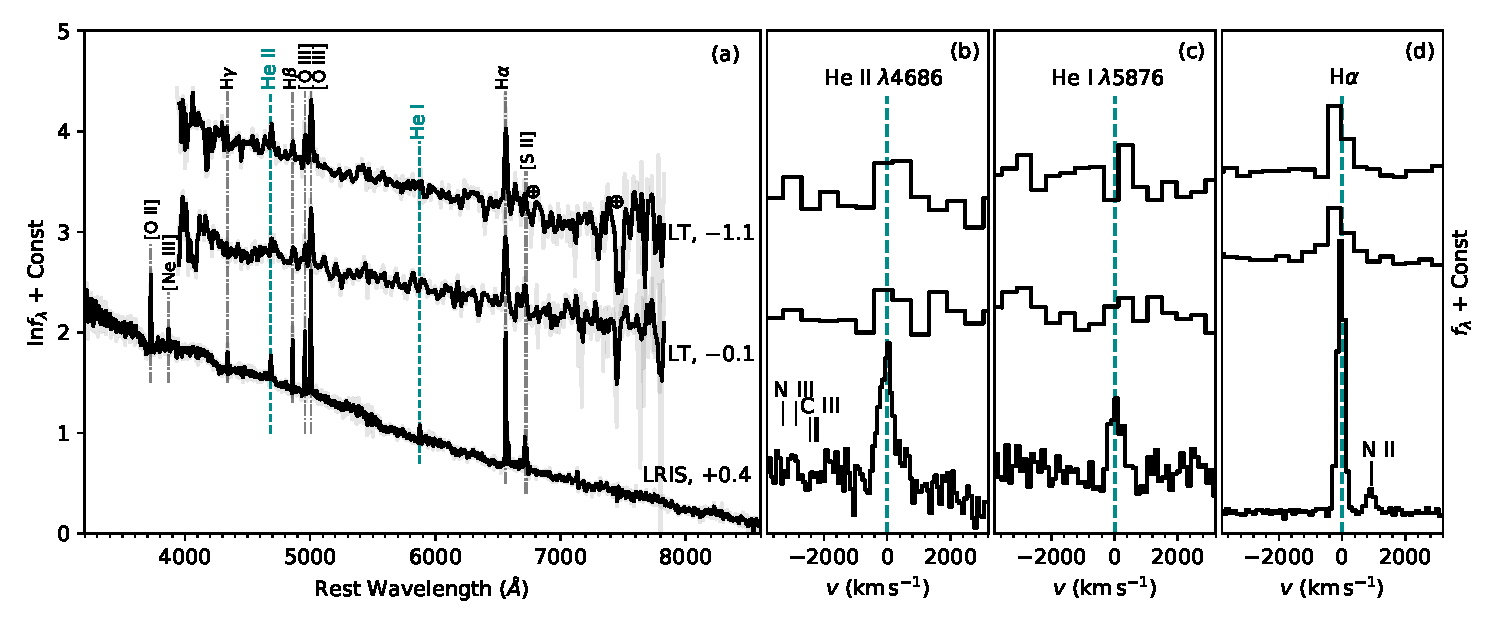
\includegraphics[width=\textwidth]{figures/spectra_early.pdf}
	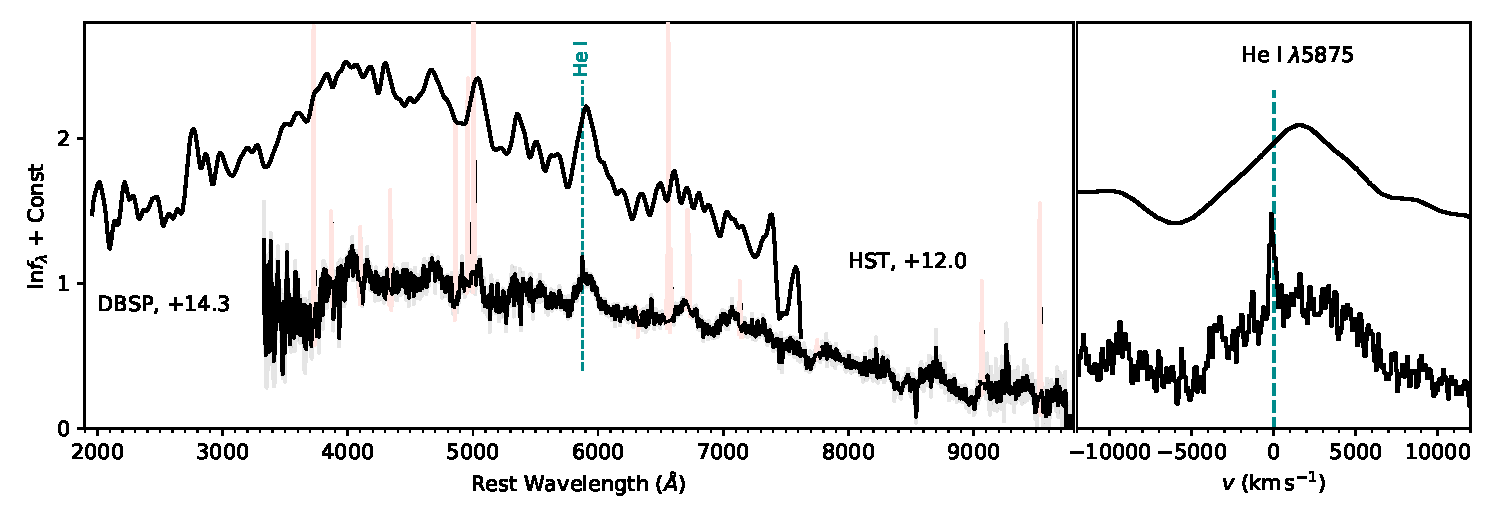
\includegraphics[width=\textwidth]{figures/spectra_phot.pdf}
	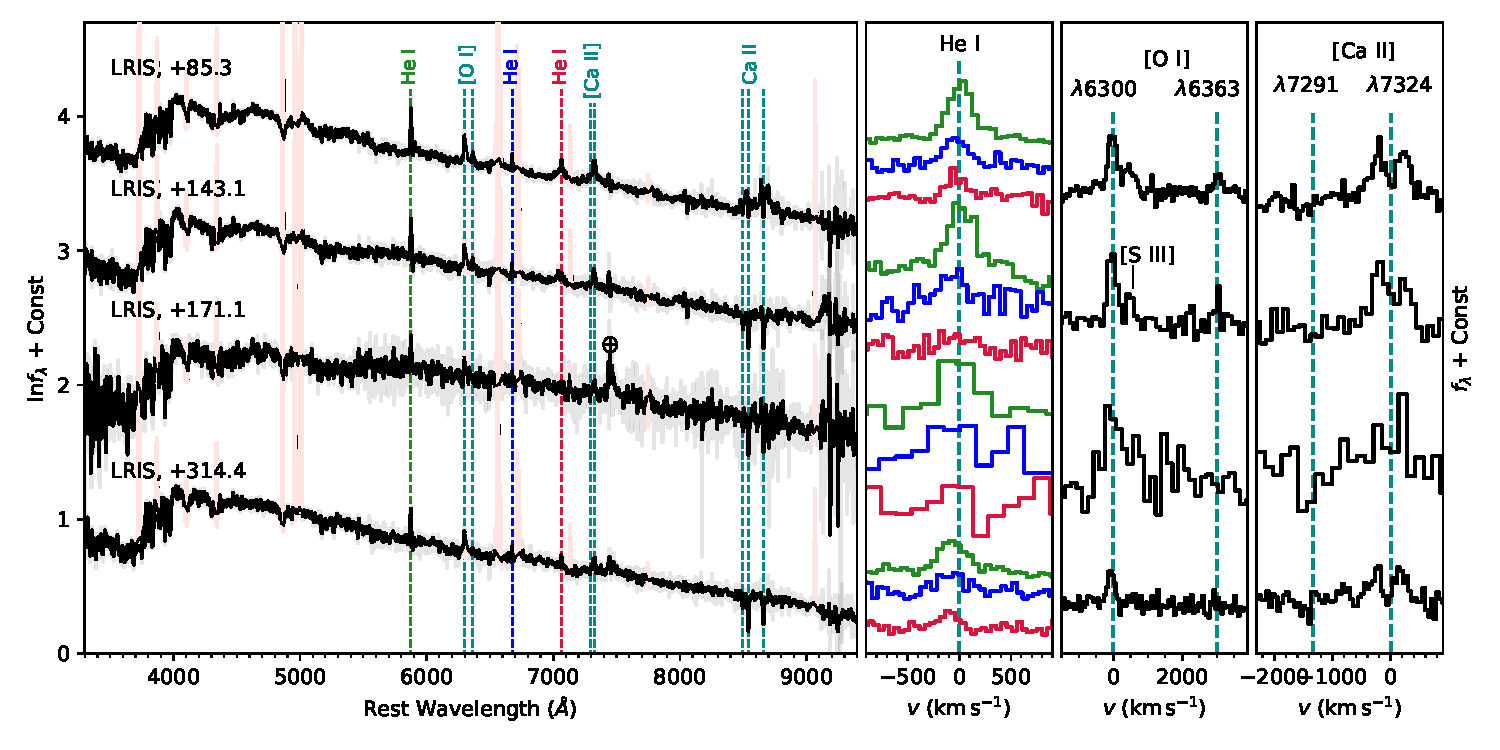
\includegraphics[width=\textwidth]{figures/spectra_late.pdf}
	\caption{Observed ealy-time spectra of AT2019dge. Prominent galaxy and SN lines are marked 
		by the vertical lines. The original spectra are shown in translucent colors, with the overlying black 
		lines showing the same spectra convolved with an ${\rm FWHM} = 800\, {\rm km\, s^{-1}}$ (for LT 
		spectra) or ${\rm FWHM} = 200\, {\rm km\, s^{-1}}$ (for DBSP and LRIS spectra) Gaussian kernel. 
	Spectral evolution in velocity space around \ion{He}{I} $\lambda5876$ line. 
		\label{fig:spectra}}
	%
\end{figure*}


The very early spectra at $-1.1$, $-0.1$, and $+0.4$\,d show a blue continuum and strong galaxy 
emision lines from the underlying \ion{H}{II} region (see Figure~\ref{fig:spectra_early}). In addition. 
these spectra also show prominent high-ionization \ion{He}{II} $\lambda4686$ narrow emission that 
later disappear. No broad 
lines are seem....

narrow lines from photoionized material in a region of undistrubed CSM exterior to the SN 
\citep{Leonard2000}

These lines were created by recombination of some CSM flash-ionized by a shock breakout 
\citep{Khazov2016} . \todo{Ask Avishay 
about interpretaton}

\todo{Using the line index definition given by \citet{Khazov2016}, we calculated the equivalent width of 
\ion{He}{II} to be $-7.56\pm 1.07$ $-2.66\pm 1.30$, and $-3.77\pm 0.16$ in the $-1.1$\,d, $-0.1$\,d, 
and $+0.4$\,d spectra.}

\begin{figure}[htbp!]
	\centering
	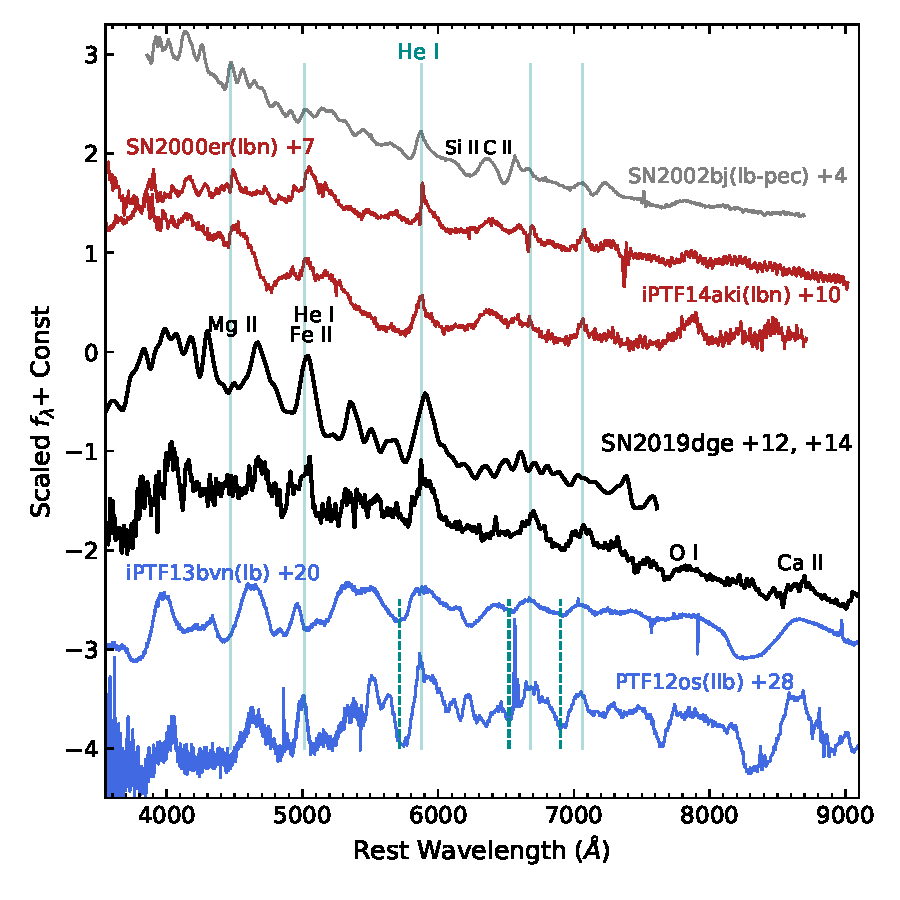
\includegraphics[width=\columnwidth]{figures/hst_opt.pdf}
	\caption{Continuum-normalized HST spectrum of AT2019dge compared with spectra of other SNe, 
	including SN2002bj \citep{Poznanski2010}, SN2005bf \citep{Folatelli2006}, SN2008ax 
	\citep{Chornock2011}, PTF12os and iPTF13bvn \citep{Fremling2016}
		\label{fig:hst_opt}}
\end{figure}
\subsubsection{Photosperic Spectral Evolution}
Broad transient features show up in the $+12.0$ adn $+14.3$\,d spectra. The existence of P-Cygni 
\ion{He}{I} $\lambda5876$ profile and non-existence of hydrogen is reminiscent of Type Ib 
SN. The HST spectrum should contain little host-galaxy contamination due to its narrow 
slitwidth and high resolution, otherwise we should see emission features at prominent galaxy line 
wavelengths (H$\alpha$, [\ion{O}{III}], [\ion{O}{II}], etc). The UV part is much weaker than a blackbody 
extrapolation opf their optical spectra would predict. This has also been seen in previous UV 
observations of SNe, and interpreted as strong metal-line blanketing, mostly by \ion{Fe}{II} and 
\ion{Co}{II} lines \citep{Gal-Yam2008}.

\todo{say that the undulations at 6700\AA is likely just noise. Ask David to put a trace on the galaxy 
center and show spectrum to get a sense of the SNR}

\begin{figure}[htbp!]
	\centering
	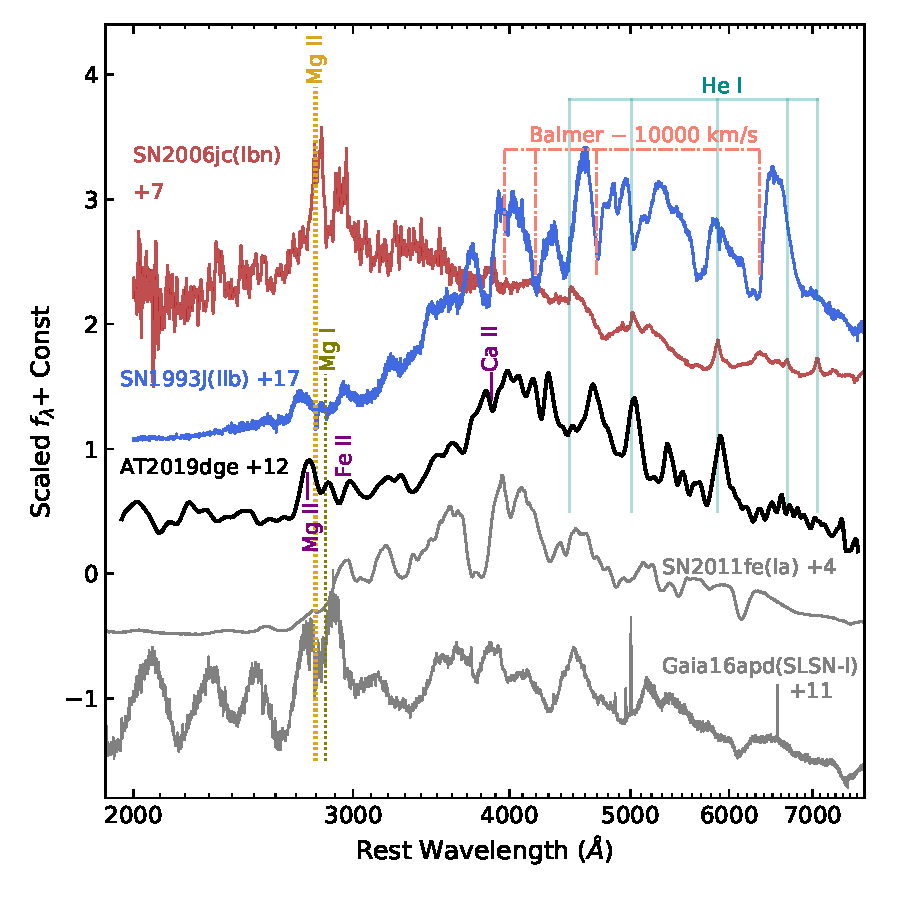
\includegraphics[width=\columnwidth]{figures/hst_all.pdf}
	\caption{HST spectrum of AT2019dge compared with spectra of other SNe, including SN2006jc 
		\citep{Bufano2009}, SN1993J \citep{Jeffery1994}, SN2011fe \citep{Mazzali2014}, and Gaia16apd 
		\citep{Yan2017}.
		\label{fig:hst_all}}
\end{figure}

In Figure~\ref{fig:hst_opt} we show that AT2019dge share similarity with those of normal SNe Ib/IIb in 
the optical region, but the spectrum does not match any known SN in 4000-4500\AA\,and 
6500--7500\AA. In Figure~\ref{fig:hst_all} we compare the HST UV spectrum too other type of SN. 
AT2019dge most closely resemble SN1993J between 2000 and 4000\AA. .

At $+12$\,d, the velocity of the \ion{He}{I} $\lambda5876$ line is $\sim7000\, {\rm km\,s^{-1}}$ 
(Figure~\ref{fig:HeI_dbsp}); At maximum light, we expect the photospheric velocity to be higher. A 
linear fit to the first few $R_{\rm bb}$ vs. time measurements (lower panel of Figure 
\ref{fig:Tbb_Rbb_Lbb}) gives $v_{\rm ej}\sim 10,000\, {\rm km\,s^{-1}}$.

\subsubsection{Late-time  Spectral Evolution}
In our late time spectrum obtained at $+85.3$, $+143.1$ and $+171.1$\,d, we observe narrow emission 
lines that are typically the most prominent features of SNe Ib/c at nebular epochs. The emission feature 
at $\sim6300$\AA\,is regularly attributed to [\ion{O}{I}] $\lambda\lambda$6300, 6364 
\citep{Maedo2008}

\ion{O}{I}, \ion{Ca}{II} and \ion{He}{I} lines. 
This feature is , and  (e.g., Maeda et al. 2008; Taubenberger et al. 
2009). The presence or absence of this feature has often been considered the sharpest observational 
discrimination between core-collapse and thermonuclear SNe (e.g., Filippenko 1997). 
the [O i] λλ6300, 6364 feature consists of two similarly strong, fairly narrow emission peaks on top of 
a broad base (figure blah blah)

In Figure \ref{fig:HeI_dbsp} we show the 
Its absorption minimum indicates a velocity of xxx

Both these transients share similarities in that they exhibit signs of interaction with H-poor 
circumstellar material (CSM) after peak, and may be the likely candidates for low energy explosions in 
dense H-poor CSM (e.g. \citealt{KleiserFuller2018, KleiserKasen2018}).

\subsection{SN location and Host Galaxy Properties}
\begin{figure}
	\centering
	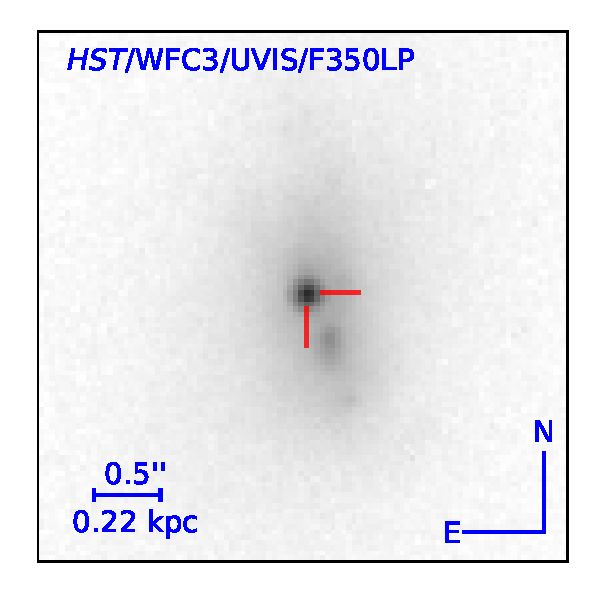
\includegraphics[width=0.8\columnwidth]{figures/offset.pdf}
	\caption{The position of AT2019dge (red crosshairs) in its host galaxy.
		Images are combined using the prescription in \citet{Lupton2004}.
		\label{fig:offset}}
\end{figure}
In Figure~\ref{fig:offset}, we show the source position on the image from the Beijing-Arizona Sky 
Survey(BASS, \citealt{Zou2017}), which is part of the DESI Legacy Imaging Surveys \citep{Dey2019}. 
Using the re-centered transient position reported in Section \ref{subsubsec:opt_phot}, we calculated 
that AT2019dge is $0.14^{\prime\prime}$ (0.06\,kpc) away from the galaxy nucleus, which is defined to 
be the flux-weighted first 
moment of the BASS $g$-band image.

Since there was no pre-explosion spectrum of the host galaxy, we estimated the host flux 
by fitting a synthetic galaxy spectrum with SDSS model magnitudes (van Velzen et al. 2019). To 
perform subtraction of the host flux, we calibrated the flux level in each optical spectrum against ZTF 
$r$-band photometry, interpolated to the spectroscopic epochs. We then convolved the synthetic 
host galaxy spectrum with a Gaussian kernel to account for instrumental broadening and subtracted 
the broadened, synthetic spectrum from our observed spectra. A montage of the host-subtracted 
spectra is shown in Figure \ref{fig:spectra}. The flux is normalized to the 5500–6000 A ̊ region in rest 
wavelength and offset from each other for better visualization.

In Fig we shoulw the SED of xx, which was compiled from Swfit/UVOT, SDSS, and catalogs and 

We measure the metallicity of the host galaxy using  the spectrum xx. 

We infer a star-formation rate of $0.10 \pm 0.02 \, M_\odot\, {\rm yr^{-1}}$ from the H$\alpha$ 
emission line using the \citet{Kennicutt1998} relation converted to use a Chabrier initial mass function 
\citep{Chabrier2003, Madau2014}. 

We also compute the oxygen abundance using the strong-line metallicity indicator N2 
\citep{Pettini2004} with the updated calibration reported in \citet{Marino2013}. The oxygen abundance 
in the N2 scale is 8.23 $\pm$ 0.01 (stat) $\pm$ 0.05 (sys).

It is worth noting that while several 
previously reported events (SN\,2005ek, SN\,2010X, iPTF\,14gqr) and SN\,2018kzr were found in star 
forming host galaxies, SN\,2019bkc stands out as a hostless transient offset by tens of kpc from any 
likely host (see Table \ref{tab:compare}). 

%%%%%%%%%%%%%%%%%%%%%%%%%%%%%%%%%%%%%%%%%%%%%%%%%%
%%%%%%%%%%%%% COMPARISON TO PREVIOUS TRANSIENTS %%%%%%%%%%%%
%%%%%%%%%%%%%%%%%%%%%%%%%%%%%%%%%%%%%%%%%%%%%%%%%%
\section{Comparison to Other Hydrogen-Deficient Fast Transients}
\subsection{Rise and Decline timescales}

\begin{figure}[htbp!]
	\centering
	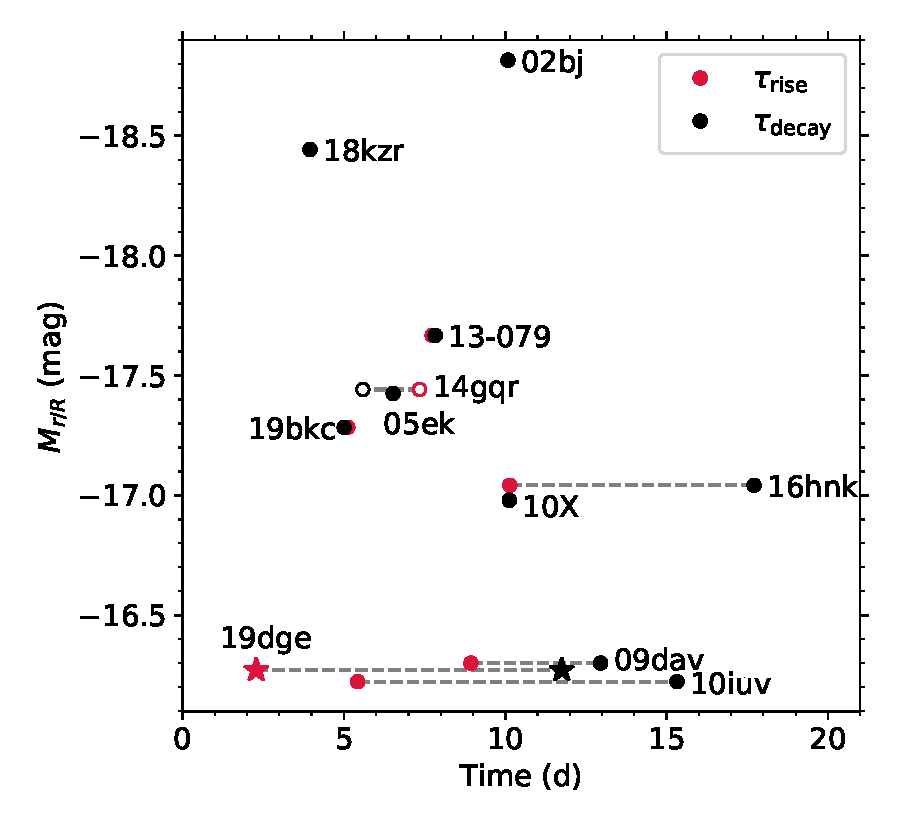
\includegraphics[width=\columnwidth]{figures/compare_mag.pdf}
	\caption{Comparison of the photometric evolution timescales ($\tau_{\rm rise}$ and $\tau_{\rm  
			decay}$) and peak absolute magnitude ($M_{r/R}$) of AT2019dge to other H-deficient fast 
			evolving 
		SNe. 
		These include 
		SN2002bj \citep{Poznanski2010},
		SN2005ek \citep{Drout2013}, 
		PTF09dav \citep{Sullivan2011}, 
		SN 2010X \citep{Kasliwal2010},
		PTF10iuv \citep{Kasliwal2012},
		OGLE-2013-SN-079 \citep{Inserra2015}, 
		iPTF14gqr \citep{De2018}, 
		SN2016hnk \citep{Galbany2019}, 
		SN2018kzr \citep{McBrien2019}, 
		SN2019bkc \citep{Chen2019}. 
		Empty circles indicate lower limits of the timescales.
		%\\ZTF $g$-band detection for SN2019bkc and ATLAS $o$-band detection for SN2016hnk. 
		\label{fig:compare_mag}}
\end{figure}

To characterize the rise and decline timescales of AT2019dge, we calculate rise time ($\tau_{\rm rise}$) 
defined by how long it takes the $r$-band light curve to rise from one magnitude below peak to peak, 
and decline time ($\tau_{\rm decay}$) determined by how long it takes to decline from peak by one 
magnitude. Figure \ref{fig:compare_mag} shows the comparison of maximum light absolute magnitude 
corrected for Galactic extinction ($M_{r/R}$), $\tau_{\rm rise}$ and $\tau_{\rm decay}$ between 
AT2019dge and other fast-evolving hydrogen-deficient transients. The peak luminosity of AT2019dge 
is lower than normal SNe Ib ($M_R\approx -17.9\pm0.9$\,mag, \citealt{Drout2011}) but consistent with 
those of the Ca-rich gap transients (e.g., PTF09dav and PTF10iuv shown in 
Figure~\ref{fig:compare_mag}), which occupy the luminosity `gap' between novae and SNe (peak 
absolute magnitude $M_R \approx -15.5$ to $-16.5$\,mag).

We conclude that AT2019dge exhibits unique differences in light curve shape (faintest $r$-band peak 
magnitude, greatest $\tau_{\rm decay}$ and the smallest $\tau_{\rm rise}$) within this set of fast 
evolving Type I events. 

The early decline of iPTF14gqr \todo{point to the figuree 4 and discuss a little bit}


\subsection{Color Evolution}
\begin{figure*}[htbp!]
	\centering
	    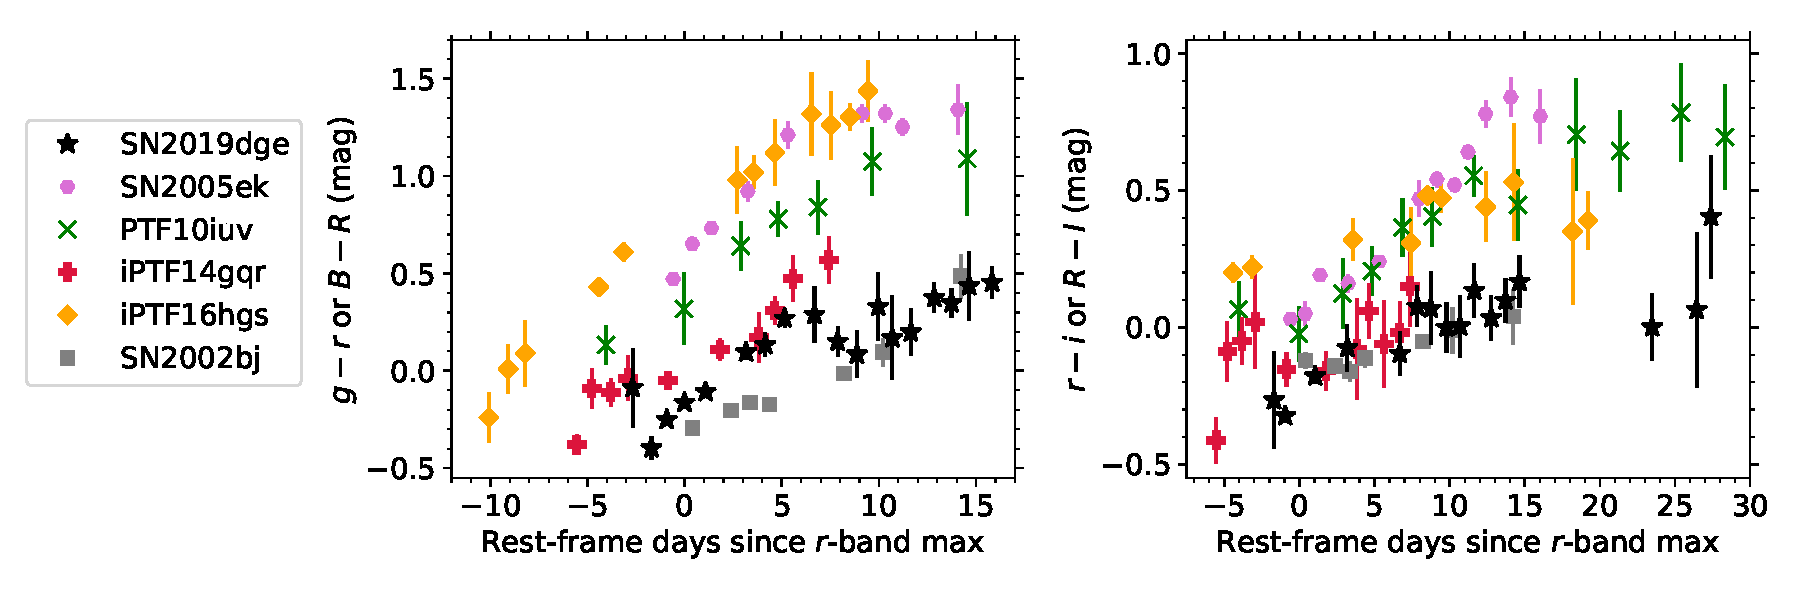
\includegraphics[width=\textwidth]{figures/compare_color.pdf}
	\caption{Comparison of the color evolution of AT2019dge with some other fast SNe shown in 
	Figure~\ref{fig:compare_mag}. All colors have been corrected for Galactic extincton. Due to absence 
	of photometry in identical filters, we compare colors in corresponding filter pairs of $B$/$g$, 
	$R$/$r$ and 
	$I$/$i$. \label{fig:compare_color}}
\end{figure*}

We compare the color curves of other fast transients to that of AT2019dge in 
Figure~\ref{fig:compare_color}, in corresponding pairs of $B$/$g-R$/$r$ and $R$/$r-I$/$i$ colors. The 
early-time blue color of AT2019dge arises from the high-temperature peak. Subsequently, AT2019dge 
has relatively typical $g-r$ color evolution among this set of transients, displaying a 
progression from a very blue transient ($g-r \approx -0.4$ mag) at early times to a relatively red 
transient ($g-r \approx 0.5$) within 10 days of explosion. This fast reddening is indicative of rapid 
cooling of the ejecta since the spectra at these phases are broadly consistent with featureless 
continua. We conclude that the multi-color light curves of the main peak of iPTF 14gqr exhibit several 
similarities (light curve shape and timescales) as well as unique differences (short rise time) in this 
sample of transients.

AT2019dge shows a color starting out blue and turning redder with time, consistent with an expanding 
and cooling photosphere.

Although AT2019dge has the same optical peak luminsity as Ca-rich transients, their multi-color light 
curves of are very different in shape. The color evolution  which otherwise form a fairly homogeneous 
class. 

\todo{AT2019dge is special in that the color even turned green a littble bit at $6<\Delta t<10$.}

We 
also searched for analogues of AT2019dge in samples of rapidly evolving events at high-redshift, 
including Pan-STARRS1 Medium Deep Survey (PS1-MDS. \citealt{Drout2014}) and the Dark Energy 
Survey (DES \citealt{Pursiainen2018}). 

Of the 10 PS1-MDS objects with spectroscopic redshift, PS1-10ah

Of the DES sample, 

% the Subaru Hyper Suprime-Cam Transient Survey (HSC, \citealt{Tanaka2016}), very few data that I 
% can compare to, remove this.

\subsection{Spectroscopy}

Although there is a large diversity in the properties of these events, most of them can be 
grouped into events that are similar to thermonuclear SNe (e.g. PTF09dav, \citealt{Sullivan2011}; 
OGLE-2013-SN-079, \citealt{Inserra2015}; SN2016hnk, \citealt{Galbany2019, Jacobson-Galan2019}) 
likely arising from old white dwarfs, and those similar to Type Ib/c SNe (SN\,2002bj, 
\citealt{Poznanski2010}; SN\,2005ek, \citealt{Drout2013}; SN\,2010X, \citealt{Kasliwal2010}; iPTF\,14gqr, 
\citealt{De2018}) possibly arising from extremely stripped massive stars or white dwarfs in close binary 
systems.

Ca-rich transients have detectable [O I] λλ6300, 6364 emission in nebular spectra, but a defining 
feature of the class is an integrated [Ca II]/[O I] flux ratio greater than ∼2. 

\subsection{Host Environment}

Table \ref{tab:compare} shows a summary of our literature search.

\begin{deluxetable*}{lllll}[htbp!]
	\tablecaption{Summary of Subluminous Fast Transient. \label{tab:compare}}
	\tablehead{
		\colhead{Name}   
		& \colhead{Redshift} 
		& \colhead{Host} 
		& \colhead{Offset (kpc)}   
		& \colhead{Reference}   
	}
	\startdata
	SN\,2002bj & 0.012   & NGC 1821 (small barred irregular galaxy, $D\sim$1.1'') & 1.8\,kpc \\
	SN\,2005ek & 0.016 & UGC 2526 (edge-on spiral galaxy of morphology Sb) & 30\,kpc \\
	% SN 2007ax, from the SDSS image, I think it is 5 arcsec from the host
	SN\,2007ax & 0.007  & NGC 2577 (small lenticular galaxy with a condensed core) &1.0\,kpc 
	\\
	PTF\,09dav & 0.036& spiral galaxy & $\sim40.6$\,kpc\\
	SN\,2010X &  0.015  & NGC 1573A (small spiral galaxy, $D\sim$1.6'') & 2.3\,kpc\\
	%PTF\,10iuv & 0.025?   &  Galaxy cluster with early-type and late-type galaxies   & $\geq 37$\,kpc  \\
	OGLE13-079 & $\sim$0.07  & in the extreme outskirts of two ellipticals & 40.2--49.9\,kpc \\
	iPTF\,14gqr & 0.063 & IV Zw 155 (a tidally interacting spiral galaxy) & 29\,kpc & \citet{De2018} \\
	SN\,2016hnk & 0.016 & MCG-01-06-070 (Sb-type galaxy)  & 3.71 & \citet{Galbany2019}\\
	% SN2018kzr (ZTF18adaykvg), host is SDSS J082853.50$+$010638.6, offset D = d_A \times \theta = 
	%d_L / (1+z)^2 \times \theta
	SN\,2018kzr & 0.053  &  SDSS J082853.50$+$010638.6 (star forming galaxy)   &  0.6 & 
	\citet{McBrien2019}\\
	SN\,2019bkc & $\sim$0.02   & maybe NGC 3090 (giant elliptical in the MKW1 galaxy group) 
	&$\sim94.6$ & \citet{Chen2019}  \\
	AT2019dge & 0.021 & SDSS J17$+$50 (small) & 0.06 kpc & This work \\
	%ZTF\,18abkmbpy & 0.029 (129\,Mpc) &  &   kpc \\
	\enddata
	%\tablecomments{Reference: SN\,2019bkc \citep{Prentice2019}, iPTF\,14qgr \citep{De2018}, 
	%OGLE13-079 \citep{Inserra2015}, SN\,2002bj 
	%\citep{Poznanski2010}, SN\,2010X \citep{Kasliwal2010}, SN\,2016hnk \citep{Galbany2019}, 
	%AT\,2018dge (Yao in prep), SN\,2005ek \citep{Drout2013}.}
\end{deluxetable*}


\section{Interpretation}
\subsection{Radioactivity-powered SN} \label{subsec:radioactivity}
SNe light cuves are mainly powered by shock energy or radiative diffusion from a heating 
source. If the observed rise in bolometric luminsity is due to a diffusion process, we can estimate the 
ejecta mass ($M_{\rm ej}$) of AT2019dge from its rise time ($t_{\rm peak}$). \citet[][hereafter 
KK19]{Khatami2019} shows that (Eq.~23 of KK19):
\begin{align}
    \frac{t_{\rm peak}}{t_{\rm d}} = 0.11\,{\rm ln} \left( 1 + \frac{9t_s}{t_d} \right)+ 0.36. \label{eq:kk19_23}
\end{align}
Here $t_{\rm peak}$ is not sensitive to the specific formula of the heating function, but depends on the heating timescale ($t_s$), the spacial distribution of mixing, and the characteristic diffusion timescale expressed by
\begin{align}
    t_d = \sqrt{\frac{\kappa M_{\rm ej}}{v_{\rm ej}c}}, \label{eq:kk19_12}
\end{align}
where $v_{\rm ej}$ is the ejecta velocity. Eq.~(\ref{eq:kk19_23}) implies that as $t_s/t_d$ increases from 
$10^{-2}$ to $10^2$, $t_{\rm peak}/t_d$ only varies in a small range (from 0.4 to 1, Fig.~6 of KK19). 
Assuming $t_{\rm peak}\approx 2\,{\rm d}$, $v_{\rm ej}\approx 7000\,{\rm km\, s^{-1}}$, and $\kappa 
\sim 0.1\, {\rm cm^2\,g^{-1}}$, $t_d$ is roughly 2.3--5.4\,d. Using Eq.~(\ref{eq:kk19_12}), $M_{\rm ej}$ is 
estimated to be 0.004--0.023\,$M_{\odot}$. 

We first examine if the peak of AT2019dge is likely to be powered by the radioactive decay of $^{56}\rm 
Ni \rightarrow ^{56}Co \rightarrow ^{56}Fe$. The energy deposition rate is
\begin{align}
    \varepsilon_{\rm rad} =
    &\varepsilon_{\rm Ni, \gamma} (t) + \varepsilon_{\rm Co, \gamma} (t)  \; {\rm [erg\,g^{-1}\,s^{-1}]}\\
 \varepsilon_{\rm Ni, \gamma} (t)   =& 3.9 \times 10^{10} e^{-t/t_{s, {\rm Ni}}}  \\
\varepsilon_{\rm Co, \gamma} (t)     &= 7\times 10^{9} \left( e^{-t/t_{s, {\rm Co}}} - e^{-t/t_{s, {\rm Ni}}}\right)
\end{align}
where $t_{s, {\rm Ni}}=8.8$\,d and $t_{s, {\rm Co}}=111.3$\,d are the decay lifetimes of $^{56}\rm Ni$ and $^{56}\rm Co$ \citep{Nadyozhin1994}. The effective heating rate is modified by the probability of thermalization, and thus $\varepsilon_{\rm heat} \leq \varepsilon_{\rm rad}$.

For $^{56}\rm Ni$ powered explosions, the bolometric light curve can be generally divided into the photospheric phase and the nebula phase. Early observations at the photospheric phase are commonly used to constrain parameters such as the explosion epoch, the total nickle mass ($M_{\rm Ni}$) and the explosion energy. Recently, KK19 presents improved analytic relations (compared with the original \citealt{Arnett1982} model) between $t_{\rm peak}$ and $L_{\rm peak}$. When $t<10$\,d, $\varepsilon_{\rm Ni}(t) \gg \varepsilon_{\rm Co}(t)$, and thus we have an exponential heating function 
\begin{equation}
    L_{\rm heat}(t) = L_0 e^{-t/t_{s, {\rm Ni}}}
\end{equation}
where $L_0 = M_{\rm Ni}\cdot \varepsilon_{\rm Ni, \gamma}$. In this case, KK19 (Eq.~21) shows that the 
relation between peak time and luminosity is:
\begin{equation}
    L_{\rm peak} = \frac{2L_0 t_s^2}{\beta^2 t_{\rm peak}^2} \left[ 1 - (1 + \beta t_{\rm peak}/t_s ) e^{-\beta t_
    {\rm peak}/ t_s} \right]
\end{equation}
where $\beta \sim 4/3$ gives a reasonable match to numerical simulations. Adopting $L_{\rm 
peak}\approx 5\times 10^{42}\,{\rm erg \, s^{-1}}$, we get an estimate of $M_{\rm Ni}\sim 
0.08 M_{\odot}$. Since $M_{\rm ej}$ is much smaller than the nickle mass needed to 
power the peak luminosity, we conclude that the peak of AT2019dge is not powered by radioactivity. 

\begin{figure}
	\centering
	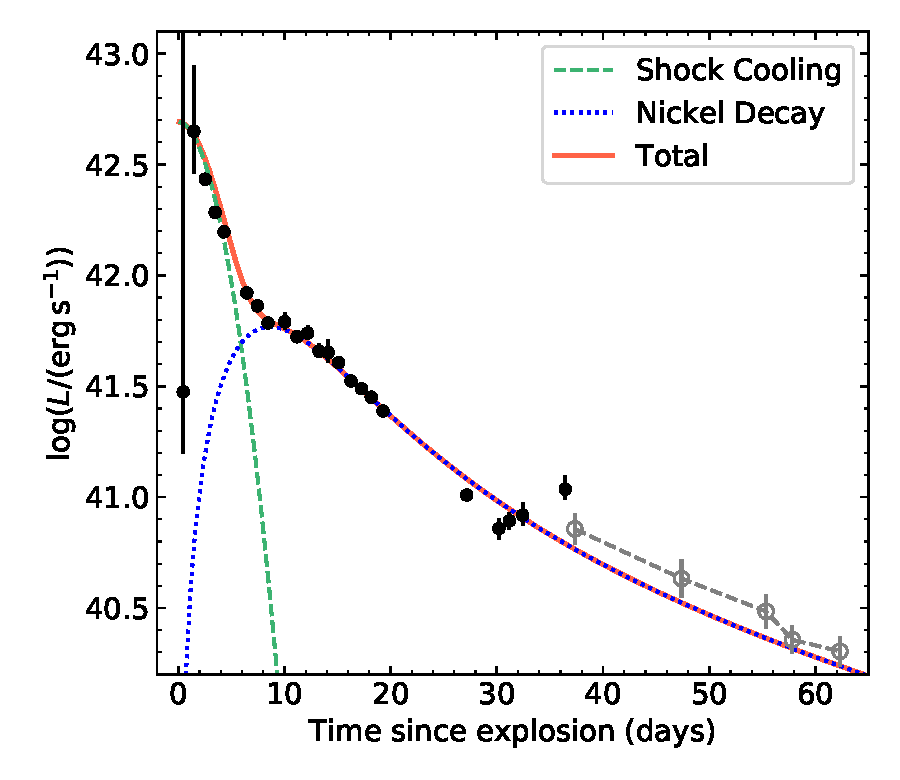
\includegraphics[width=\columnwidth]{figures/Lbb.pdf}
	\caption{Bolometric light curve for AT2019dge. The quasi-bolometric light curve of AT2019dge 
	estimated by computing $\nu L_\nu$ in $r$-band is shown as emply circles.}
	\label{fig:Lbb}
\end{figure}

Next, we examine wheter the late time light curve can be powered by $^{56}\rm Ni$ decay. At the 
nebula phase the SN ejecta becomes optically thin, such that the delay between the energy deposition 
from radioactivity and the optical radiation becomes shorter. The bolometric luminosity is then equal to 
the rate of energy deposition: $L_{\rm bol}(t) = Q(t)$. At any given time, the energy deposition rate 
$Q(t)$ is \citep{Wygoda2019}:
\begin{align*}
    Q(t) = Q_{\gamma}(t)\left( 1 - e^{-(t_0/t)^2}\right) + Q_{\rm pos}(t),
\end{align*}
where $Q_{\gamma}(t) = M_{\rm Ni}\varepsilon_{\rm rad}$ is the energy release rate of gamma-rays and $t_0$ is the time at which the ejecta becomes optically thin to gamma rays. $Q_{\rm pos}(t)$ is the energy deposition rate of positron kinetic energy:
\begin{align}
Q_{\rm pos}(t) &= M_{\rm Ni}\varepsilon_{\rm Co, pos}(t)\\
    \varepsilon_{\rm Co, pos}(t) &=  2.3\times 10^{8} \left( e^{-t/t_{s, {\rm Co}}} - e^{-t/t_{s, {\rm Ni}}}\right)
\end{align}

In Figure~\ref{fig:Lbb}, bolometric light curve measured in Section \ref{subsec:lc_properties} are shown 
in black. We also show late-time $r$-band $\nu L_{\nu}$ measurements in grey empty circles as a 
proxy of bolometric light curve evolution. Model tracks with $t_0 = 40$\,d and $M_{\rm Ni} =0.004$, 
0.008, and 0.02$M_\odot$ are plotted in blue lines. From Figure~\ref{fig:Lbb}, it is evident that the late 
time `tail' can be explained by a continuing input of decay energy with $M_{\rm Ni}\sim 0.008 M_\odot$ 
and $t_0~40$\,d. 

Assuming that radioactivity dominates the light curve after the initial abrupt drop of bolometric 
luminosity ($t>10$\,d). If the nebula phase starts 20--25 days after explosion, we use the above 
equations to constrain model parameters to be $M_{\rm Ni} = 
0.008 \pm 0.001 \,M_\odot$ and $t_0 = 39.0^{+4.5}_{-4.7}$\,days. The photospheric phase can be 
modelled using Equations given in \citet[][Appendix A]{Valenti2008}, with modifications given by 
\citet[][Eq.~3]{Lyman2016}, where the light curve shape is determined by $M_{\rm Ni}$ and the photon 
diffusion time $\tau_{\rm m}$. In Figure~\ref{fig:Lbb} we overplot this photospheric model fit by eye in 
dotted cyan line. We are unable to achieve an excellent match to data between $t=10$\,d and 
$t=20$\,d. This may be explained by inaccuracy of the Arnett solution, but more likely due to other 
emission mechanisms contributing a non-negligible amount of radiation at this early phase.

\subsection{Shock Cooling Emisssion} \label{subsec:shock}
We model the early light curve as cooling emission from shock-heated extended material using models 
presented by \citet[][hereafter P15]{Piro2015} to constrain the mass and radius of the extanded material
($M_{\rm ent}$ and $R_{\rm ent}$, respectively). Details of the model fitting to multi-band observations 
are illustrated in Appendix \ref{subsec:p15fit}. This model is built on analytical results of 
\citet{Nakar2014}, and $M_{\rm ext}$ includes only mass concentrated around $R_{\rm ext}$. In 
Figure~\ref{fig:envelope}, we show the best-fitting model of $M_{\rm env} = 9.40_{-0.33}^{+0.69}\times 
10^{-2} M_\odot$, $R_{\rm env} =2.69_{-0.16}^{+0.34}\times10^{12}$\,cm (i.e., $38.7_{-2.4}^{+4.9} 
R_\odot$), and first light epoch at phase $t_{\rm fl}= -3.20_{-0.04}^{+0.03}$\,day.

\begin{table}[!htbp] 
	\centering 
	\caption{shock P15.} 
	\begin{tabular}{ccll} 
		\hline 
		Name  &Type & $R_{\rm ext}$ ($10^{12}\,{\rm cm}$) & $M_{\rm ext}$ ($10^{-2} M_\odot$)  \\ 
		\hline
		iPTF16hgs & Ca-rich & $0.9$ & 8\\
		\textbf{AT2019dge} & Ib-pec & $2.69_{-0.16}^{+0.34}$ & $9.40_{-0.33}^{+0.69}$  \\
		iPTF14gqr & Ic-pec &$30^{+3}_{-3}$ &$0.88^{+0.08}_{-0.07}$  \\
		iPTF15dtg & Ic & 83&5 \\
		SN2016gkg & IIb &$4.00^{+0.05}_{-0.05}$ &$2.50^{+0.01}_{-0.01}$  \\
		ZTF18aalrxas & IIb & $73^{+3}_{-2}$  & $4.3_{-0.13}^{+0.14}$ \\
		\hline 
	\end{tabular} 
\tablecomments{Reference: iPTF14gqr \citep{De2018}, SN2016gkg \citep{Arcavi2017}, 
ZTF18aalrxas\citep{Fremling2019}}
	\label{tab:bbfit} 
\end{table} 


\citet[][hereafter N16]{Nagy2016} modeled emission from the shock heated star by considering 
density profiles consisting of a compact constant-density inner ``core'' and an outer ``shell'' with 
density power law index $n$. Emission of the shell and core are independent of each other. 

As an attempt to fit the whole light curve of AT2019dge, we ignore 
recombination, fix $n=2$, thomson scattering opacity $\kappa=0.2\,{\rm cm^2\,g^{-1}}$, $M_{\rm 
Ni}=0.08\,M_\odot$ and the gamma-ray leakage parameter at $A_\gamma = t_0^2 = 1600\,{\rm day^2}$.

\begin{figure}[htbp!]
	\centering
	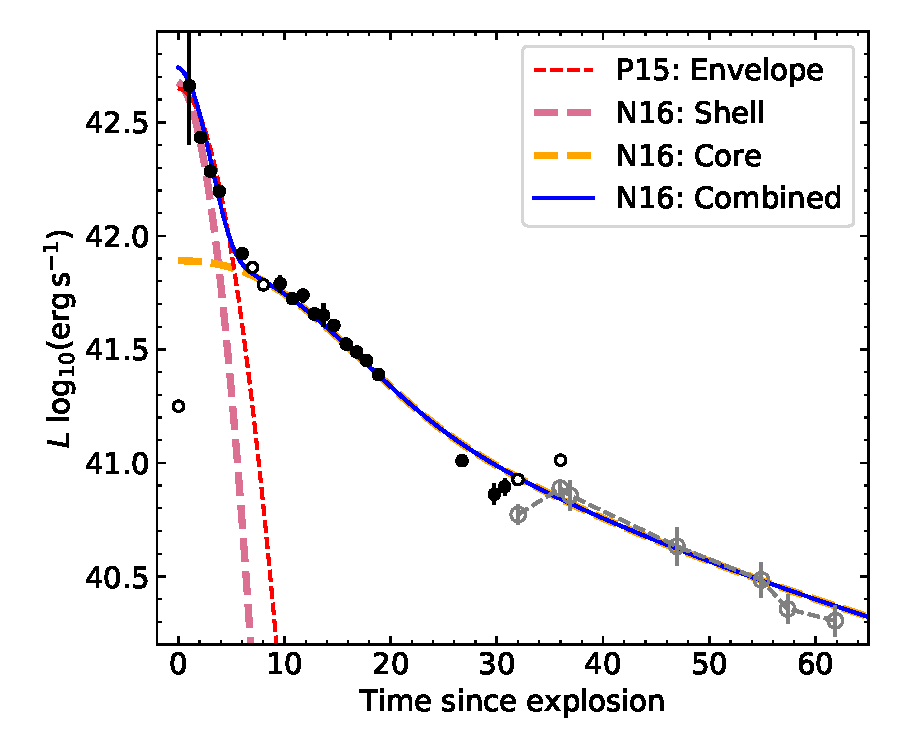
\includegraphics[width=\columnwidth]{figures/envelope.pdf}
	\caption{Cooling emission model fit to the early light curve of AT2019dge. 
		\label{fig:envelope}}
\end{figure}

\todo{This must be really shallow Ni deposit?}

%\subsection{Magnetar-powered SN}
%To test models with additional energy from a central engine, we attempt a magnetar spin-down 
%component proposed by \citet{Kasen2010} and further generalized for lightcurve fitting by 
%\citet{Inserra2013}\footnote{\url{https://star.pst.qub.ac.uk/webdav/public/ajerkstrand/Codes/Genericarnett/}}.
%We found a reasonable fit which implied an ejecta mass of 0.1Me, along with an initial magnetar spin 
%period of $P = $ and magnetic field srength of $B=$ G. 

\section{Discussion}
massive mass-loss episode that takes place just prior to the explosion \citep{Shiode2014}

Progenitor: why so rare???
Could the progenitor be a helium rich WR star, perhaps recently transitioned from an LBV phase 

Constraints on event rate?

\section{Conclusion}
In this paper we have presented observations and modeling of the fast transient AT2019dge. We 
summarize our primary observational findings below:
\begin{itemize}
	\item Peak absolute magnitude of MB = −dd mag and decline parameter of hah mag.
	\item  Total Nickel and ejecta masses of $M_{\rm Ni} = 0.03 \pm 0.01$ and $Mej = 0.9 \pm 0.3 
	M_\odot$, respectively.
\end{itemize}


Despite the steady increase in the number of events in the class of sub-luminous transients, the total 
number of well-studied events remain still small ($\approx 10$). An all-sky two-day cadence survey 
with ZTF Phase II is ideally positioned to probe this rare population over a sufficiently large volume 
(given the deeper limiting magnitude of ZTF compared to other ongoing time domain surveys) to 
address questions regarding their intrinsic properties such as luminosity functions, spectroscopic 
diversity and ejecta mass distributions of the different sub-types and their volumetric rates. As likely 
tracers of the end points of white dwarfs and massive stars in extreme binary systems, their intrinsic 
rates are not only important from the point of view of understanding these rare transient phenomena 
but also have direct implications for current and future experiments in the field of gravitational wave 
astronomy. With a higher cadence than the nominal 3-day public survey in Phase I, the 2-day cadence 
in $g$ and $r$ bands will be particularly sensitive to the population of fastest transients in the local 
universe, of which only a handful are known, while the two-color coverage will also be a powerful 
diagnostic of the intrinsic color of these events.


\acknowledgements

%% Y. Yao thanks the instructors and organisers of the GROWTH summer school for teaching 
%%essential skills in time-domain data analysis.
%% discussion with Wenbin Lu, Udi Nakar, Nathan Smith, Yan Lin, Christoffer, Fremling, Avishay
%% Jim, Sterl, Tony, Chuck?
This study made use of the open supernova catalog \citep{Guillochon2017}

\software{
          \texttt{astropy} \citep{Astropy-Collaboration13},
          \texttt{scipy} \citep{Jones01}, 
          \texttt{matplotlib} \citep{Hunter07},
          \texttt{pandas} \citep{McKinney10},
          \texttt{emcee} \citep{Foreman-Mackey2013},
          \texttt{corner} \citep{Foreman-Mackey16}
          }

%% For this sample we use BibTeX plus aasjournals.bst to generate the
%% the bibliography. The sample63.bib file was populated from ADS. To
%% get the citations to show in the compiled file do the following:
%%
%% pdflatex sample63.tex
%% bibtext sample63
%% pdflatex sample63.tex
%% pdflatex sample63.tex

\clearpage
\appendix

\section{UV and Optical Photometry} \label{app:phot}
\subsection{Data}
In Figure \ref{fig:seds} we show the photometry interpolated onto common epochs, and fit to a blackbody function to derive the photospheric evolution (Section ). The full set of photometry is listed in Table \ref{tab:phot}.
\begin{figure*}
    \centering
    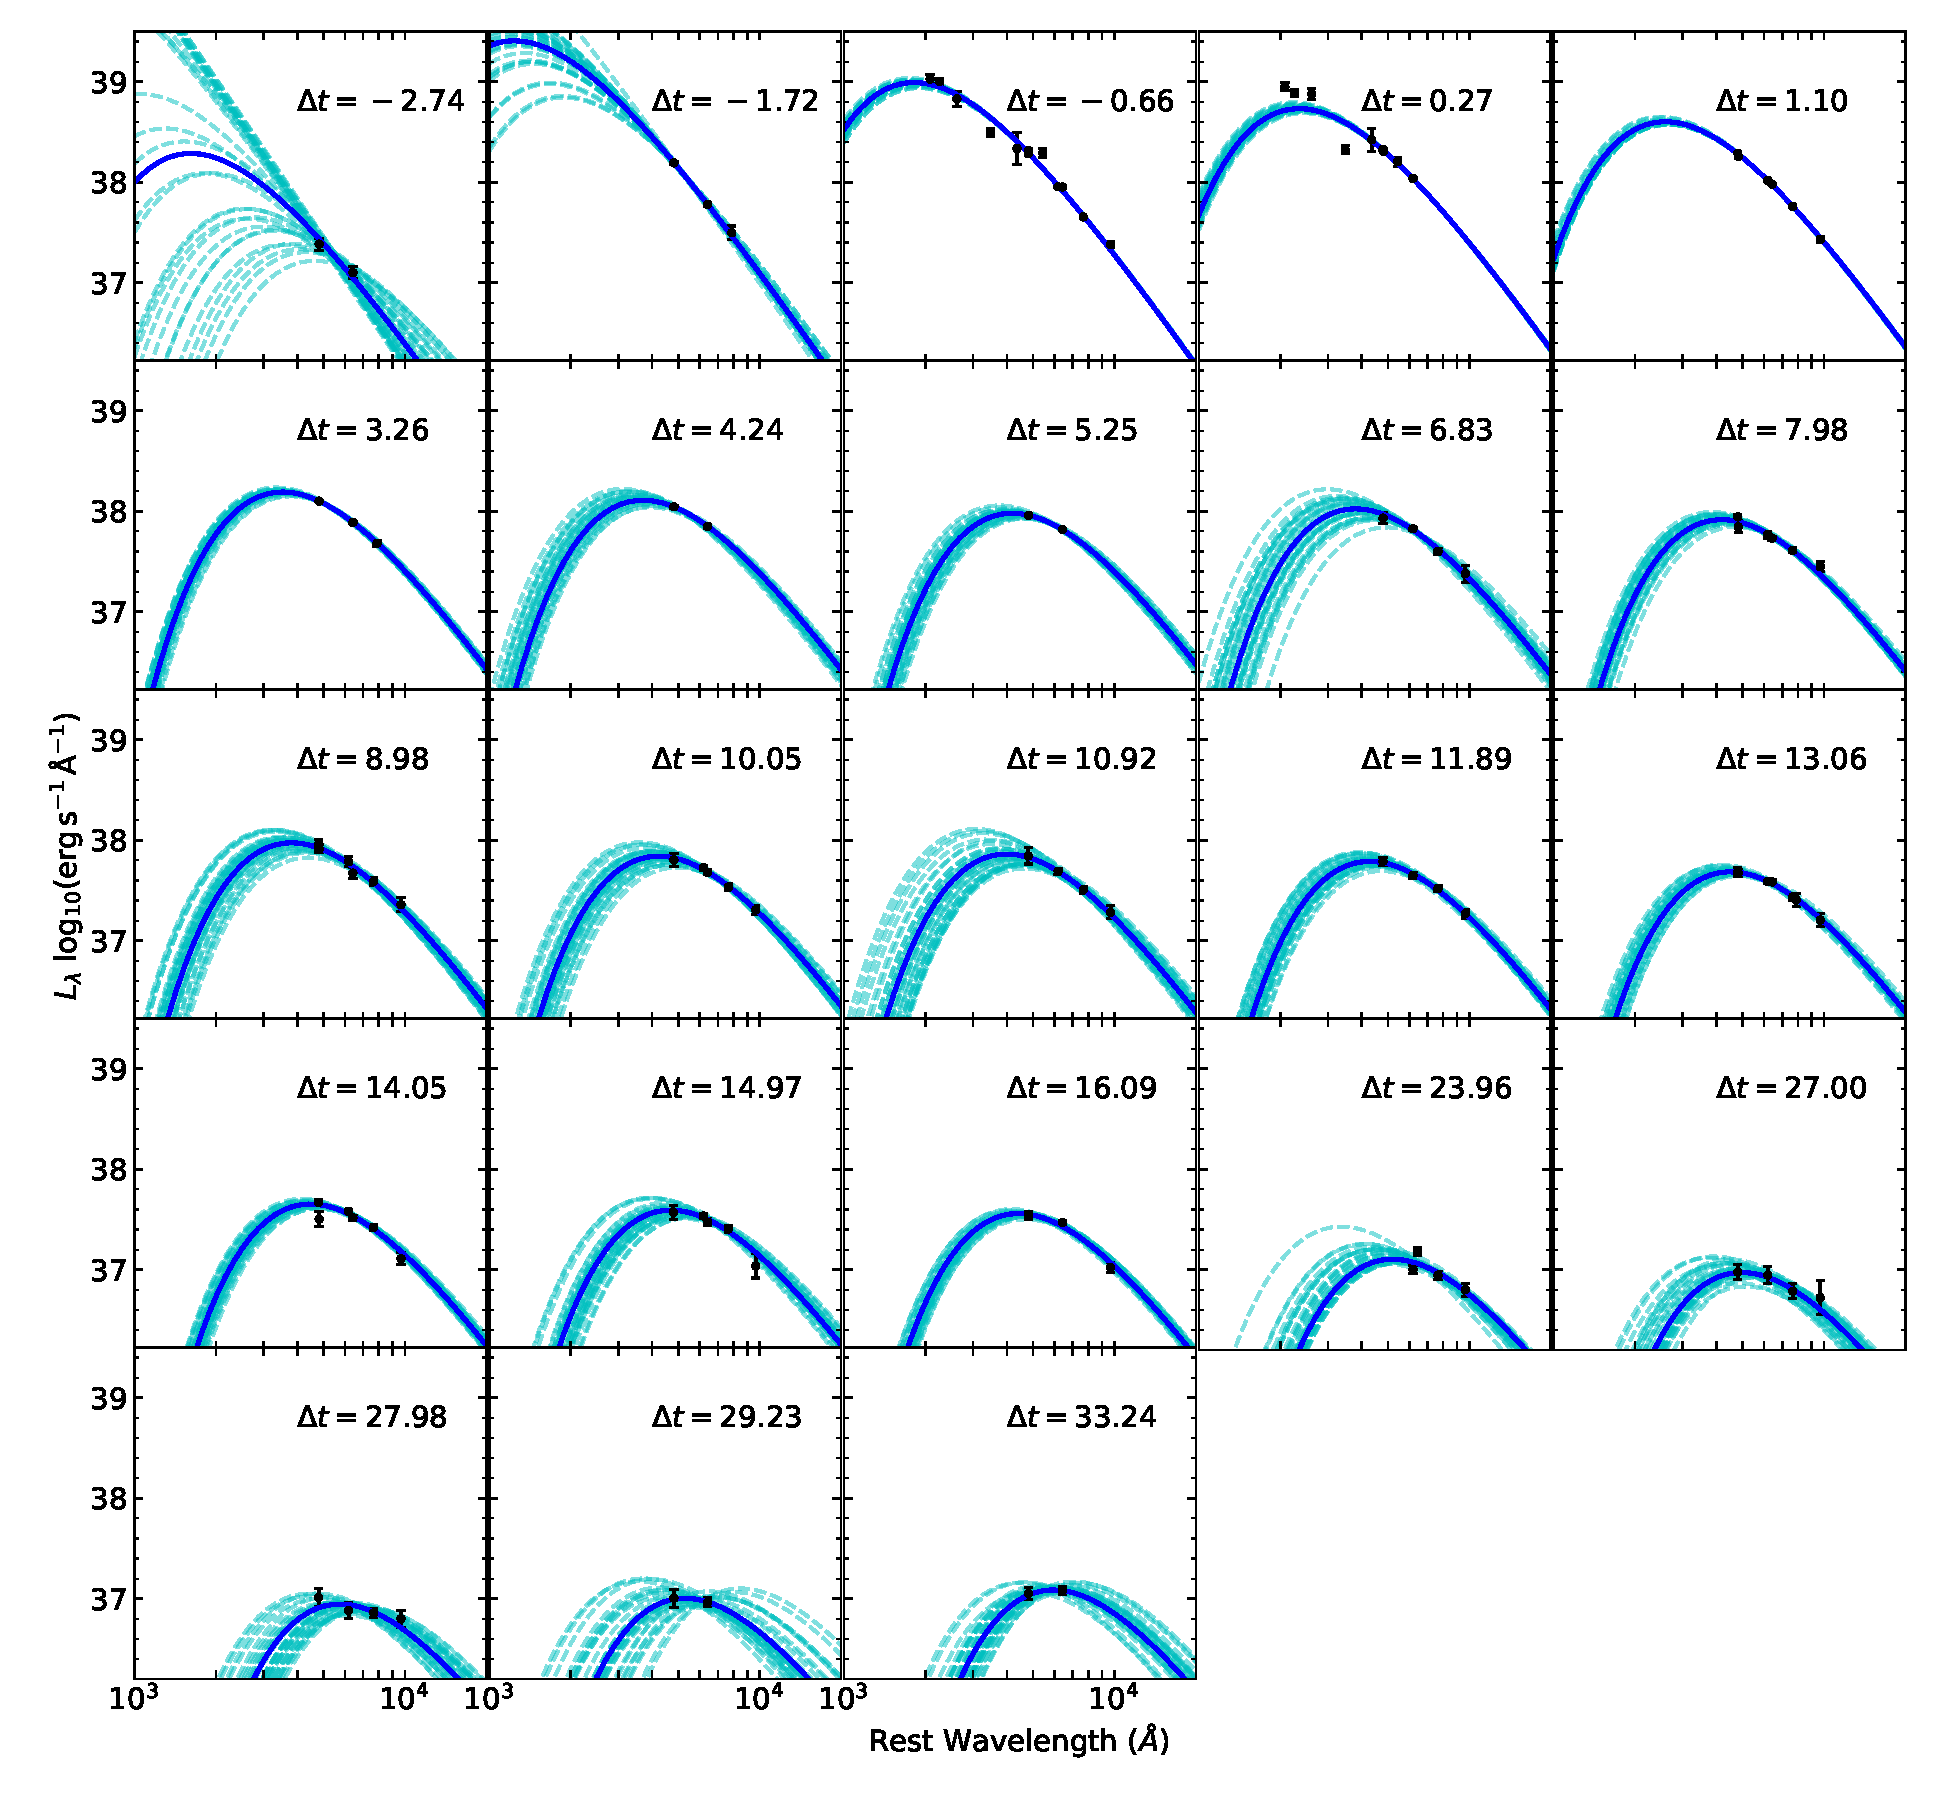
\includegraphics[width = 0.9\textwidth]{figures/seds.pdf}
    \caption{The maximum MCMC a posteriori model fits to $Swift$/UVOT and optical photometry for 
    AT2019dge.  \label{fig:seds}}
\end{figure*}

\startlongtable
\begin{deluxetable}{llllll}
\tabletypesize{\scriptsize}
\tablecaption{Optical and UV photometry for AT2019dge.\label{tab:phot}}
\tablehead{
\colhead{Date (JD)}   
& \colhead{Instrument}
& \colhead{Filter}  
& \colhead{$m$} 
& \colhead{$\sigma_{m}$}
}
\startdata
58582.1544 & LT$+$IOO & $g$ & 18.59 & 0.01 \\
58582.1552 & LT$+$IOO & $r$ & 18.84 & 0.02 \\
58582.1575 & LT$+$IOO & $i$ & 19.11 & 0.02 \\
58582.1583 & LT$+$IOO & $z$ & 19.28 & 0.07 \\
58583.1637 & LT$+$IOO & $g$ & 18.48 & 0.02 \\
58583.1645 & LT$+$IOO & $r$ & 18.63 & 0.01 \\
58584.2324 & LT$+$IOO & $g$ & 18.58 & 0.01 \\
58584.2332 & LT$+$IOO & $r$ & 18.68 & 0.02 \\
58584.2355 & LT$+$IOO & $i$ & 18.85 & 0.02 \\
58584.2363 & LT$+$IOO & $z$ & 19.15 & 0.07 \\
58590.0252 & LT$+$IOO & $g$ & 19.47 & 0.14 \\
58590.0260 & LT$+$IOO & $r$ & 19.16 & 0.04 \\
58590.0268 & LT$+$IOO & $i$ & 19.24 & 0.07 \\
58590.0277 & LT$+$IOO & $z$ & 19.28 & 0.21 \\
58591.0676 & LT$+$IOO & $g$ & 19.44 & 0.07 \\
58591.0685 & LT$+$IOO & $r$ & 19.31 & 0.09 \\
58591.0693 & LT$+$IOO & $i$ & 19.22 & 0.06 \\
58591.0701 & LT$+$IOO & $z$ & 19.10 & 0.12 \\
58592.0472 & LT$+$IOO & $g$ & 19.40 & 0.13 \\
58592.0472 & LT$+$IOO & $r$ & 19.26 & 0.12 \\
58592.0489 & LT$+$IOO & $i$ & 19.27 & 0.10 \\
58592.0497 & LT$+$IOO & $z$ & 19.33 & 0.17 \\
58593.1109 & LT$+$IOO & $r$ & 19.41 & 0.06 \\
58593.1117 & LT$+$IOO & $i$ & 19.41 & 0.08 \\
58593.1125 & LT$+$IOO & $z$ & 19.46 & 0.12 \\
58594.1142 & LT$+$IOO & $g$ & 19.69 & 0.20 \\
58594.1150 & LT$+$IOO & $r$ & 19.50 & 0.08 \\
58594.1158 & LT$+$IOO & $i$ & 19.48 & 0.08 \\
58594.1167 & LT$+$IOO & $z$ & 19.52 & 0.16 \\
58595.0926 & LT$+$IOO & $g$ & 19.82 & 0.10 \\
58595.0935 & LT$+$IOO & $r$ & 19.60 & 0.07 \\
58595.0943 & LT$+$IOO & $i$ & 19.45 & 0.07 \\
58595.0951 & LT$+$IOO & $z$ & 19.55 & 0.11 \\
58596.1380 & LT$+$IOO & $g$ & 20.10 & 0.11 \\
58596.1388 & LT$+$IOO & $r$ & 19.75 & 0.06 \\
58596.1396 & LT$+$IOO & $i$ & 19.66 & 0.08 \\
58596.1405 & LT$+$IOO & $z$ & 19.71 & 0.16 \\
58597.1508 & LT$+$IOO & $g$ & 20.12 & 0.07 \\
58597.1516 & LT$+$IOO & $r$ & 19.77 & 0.05 \\
58597.1539 & LT$+$IOO & $i$ & 19.69 & 0.07 \\
58597.1547 & LT$+$IOO & $z$ & 19.95 & 0.15 \\
58598.1207 & LT$+$IOO & $g$ & 20.37 & 0.17 \\
58598.1218 & LT$+$IOO & $r$ & 19.89 & 0.06 \\
58598.1247 & LT$+$IOO & $i$ & 19.73 & 0.08 \\
58598.1257 & LT$+$IOO & $z$ & 20.13 & 0.30 \\
58599.1894 & LT$+$IOO & $g$ & 20.42 & 0.08 \\
58599.1918 & LT$+$IOO & $z$ & 20.17 & 0.12 \\
58601.1606 & LT$+$IOO & $i$ & 20.38 & 0.10 \\
58607.0861 & LT$+$IOO & $r$ & 21.22 & 0.11 \\
58607.0890 & LT$+$IOO & $i$ & 20.88 & 0.10 \\
58607.0900 & LT$+$IOO & $z$ & 20.72 & 0.16 \\
58610.1965 & LT$+$IOO & $g$ & 21.86 & 0.19 \\
58610.1974 & LT$+$IOO & $r$ & 21.36 & 0.21 \\
58610.1982 & LT$+$IOO & $i$ & 21.28 & 0.19 \\
58610.1990 & LT$+$IOO & $z$ & 20.92 & 0.42 \\
58611.1743 & LT$+$IOO & $g$ & 21.77 & 0.23 \\
58611.1751 & LT$+$IOO & $r$ & 21.52 & 0.19 \\
58611.1759 & LT$+$IOO & $i$ & 21.10 & 0.12 \\
58611.1767 & LT$+$IOO & $z$ & 20.72 & 0.21 \\
58580.4421 & P48$+$ZTF & $g$ & 20.83 & 0.15 \\
58581.4807 & P48$+$ZTF & $g$ & 18.81 & 0.03 \\
58582.4396 & P48$+$ZTF & $g$ & 18.50 & 0.02 \\
58583.4082 & P48$+$ZTF & $g$ & 18.52 & 0.04 \\
58584.4691 & P48$+$ZTF & $g$ & 18.65 & 0.02 \\
58586.4480 & P48$+$ZTF & $g$ & 19.04 & 0.02 \\
58587.4658 & P48$+$ZTF & $g$ & 19.18 & 0.03 \\
58588.4794 & P48$+$ZTF & $g$ & 19.39 & 0.04 \\
58591.3740 & P48$+$ZTF & $g$ & 19.68 & 0.15 \\
58592.4784 & P48$+$ZTF & $g$ & 19.50 & 0.10 \\
58593.4841 & P48$+$ZTF & $g$ & 19.78 & 0.17 \\
58596.4781 & P48$+$ZTF & $g$ & 20.11 & 0.08 \\
58597.4728 & P48$+$ZTF & $g$ & 20.53 & 0.18 \\
58599.2766 & P48$+$ZTF & $g$ & 20.47 & 0.08 \\
58612.4016 & P48$+$ZTF & $g$ & 21.78 & 0.22 \\
58616.4688 & P48$+$ZTF & $g$ & 21.66 & 0.16 \\
58580.4842 & P48$+$ZTF & $r$ & 20.89 & 0.14 \\
58581.4308 & P48$+$ZTF & $r$ & 19.19 & 0.05 \\
58582.4516 & P48$+$ZTF & $r$ & 18.76 & 0.02 \\
58584.4009 & P48$+$ZTF & $r$ & 18.69 & 0.02 \\
58585.4191 & P48$+$ZTF & $r$ & 18.75 & 0.03 \\
58586.4101 & P48$+$ZTF & $r$ & 18.92 & 0.03 \\
58587.4222 & P48$+$ZTF & $r$ & 19.02 & 0.05 \\
58588.4300 & P48$+$ZTF & $r$ & 19.10 & 0.03 \\
58589.3489 & P48$+$ZTF & $r$ & 18.99 & 0.20 \\
58591.4525 & P48$+$ZTF & $r$ & 19.31 & 0.05 \\
58592.3880 & P48$+$ZTF & $r$ & 19.46 & 0.13 \\
58593.4315 & P48$+$ZTF & $r$ & 19.44 & 0.06 \\
58596.3929 & P48$+$ZTF & $r$ & 19.68 & 0.05 \\
58597.4050 & P48$+$ZTF & $r$ & 19.85 & 0.06 \\
58598.3610 & P48$+$ZTF & $r$ & 19.96 & 0.09 \\
58599.4846 & P48$+$ZTF & $r$ & 19.97 & 0.06 \\
58600.4715 & P48$+$ZTF & $r$ & 20.08 & 0.10 \\
58605.4333 & P48$+$ZTF & $r$ & 20.73 & 0.08 \\
58607.3705 & P48$+$ZTF & $r$ & 20.69 & 0.09 \\
58608.4033 & P48$+$ZTF & $r$ & 20.64 & 0.13 \\
58612.4549 & P48$+$ZTF & $r$ & 21.23 & 0.11 \\
58616.4117 & P48$+$ZTF & $r$ & 20.94 & 0.09 \\
58617.3380 & P48$+$ZTF & $r$ & 21.02 & 0.17 \\
58627.3911 & P48$+$ZTF & $r$ & 21.58 & 0.21 \\
58635.3518 & P48$+$ZTF & $r$ & 21.95 & 0.19 \\
58581.5163 & P48$+$ZTF & $i$ & 19.44 & 0.17 \\
58586.5159 & P48$+$ZTF & $i$ & 18.98 & 0.08 \\
58596.3822 & P48$+$ZTF & $i$ & 19.66 & 0.16 \\
58637.8263 & P48$+$ZTF & $r$ & 22.27 & 0.16 \\
58642.3119 & P48$+$ZTF & $r$ & 22.40 & 0.17 \\
58582.8289 & $Swift+$UVOT & $B$ & 18.68 & 0.40 \\
58582.8280 & $Swift+$UVOT & $U$ & 18.80 & 0.10 \\
58582.8346 & $Swift+$UVOT & $UVM2$ & 18.55 & 0.07 \\
58582.8261 & $Swift+$UVOT & $UVW1$ & 18.61 & 0.19 \\
58582.8299 & $Swift+$UVOT & $UVW2$ & 18.68 & 0.11 \\
58582.8337 & $Swift+$UVOT & $V$ & 18.29 & 0.11 \\
58583.5775 & $Swift+$UVOT & $B$ & 18.46 & 0.29 \\
58583.5766 & $Swift+$UVOT & $U$ & 19.22 & 0.10 \\
58583.5833 & $Swift+$UVOT & $UVM2$ & 18.85 & 0.09 \\
58583.5747 & $Swift+$UVOT & $UVW1$ & 18.49 & 0.14 \\
58583.5785 & $Swift+$UVOT & $UVW2$ & 18.87 & 0.10 \\
58583.5823 & $Swift+$UVOT & $V$ & 18.51 & 0.11 \\
\enddata
\tablecomments{$m$ and $\sigma_m$ are observed magnitude (without extinction correction) in AB system.}
\end{deluxetable}


\subsection{Modelling Early Light Curve} \label{subsec:p15fit}
\begin{deluxetable}{llc}[htpb!]
	\tablecaption{Model Parameters $\theta$ and Their Priors \label{tab:P15priors}}
	\tablehead{
		\colhead{$\theta$}
		& \colhead{Description}
		&\colhead{Prior}
	}
	\startdata
	${\rm lg}R_{\rm ext}$ & log$_{10}$ of extented material radius in cm  & 
	$\mathcal{U}(-5, 25)$ \\
	${\rm lg}M_{\rm ext}$ &  log$_{10}$ of extented material mass in $M_\odot$  & $\mathcal{U}(-4, 0)$\\
	$t_\mathrm{fl}$ & first light epoch in MJD relative to $58583.2$& $\mathcal{U}(-8,-2.76)$ \\
	$E_{51}$ & SN energy divided by $10^{51}\,{\rm erg\,s^{-1}}$ & $\mathcal{U}(0.01, 10)$ \\
	$M_{\rm core}$ & core mass in $M_{\odot}$ & $\mathcal{U}(0.1,100)$ \\
	\enddata
\end{deluxetable}

\begin{figure}[htbp!]
	\centering
	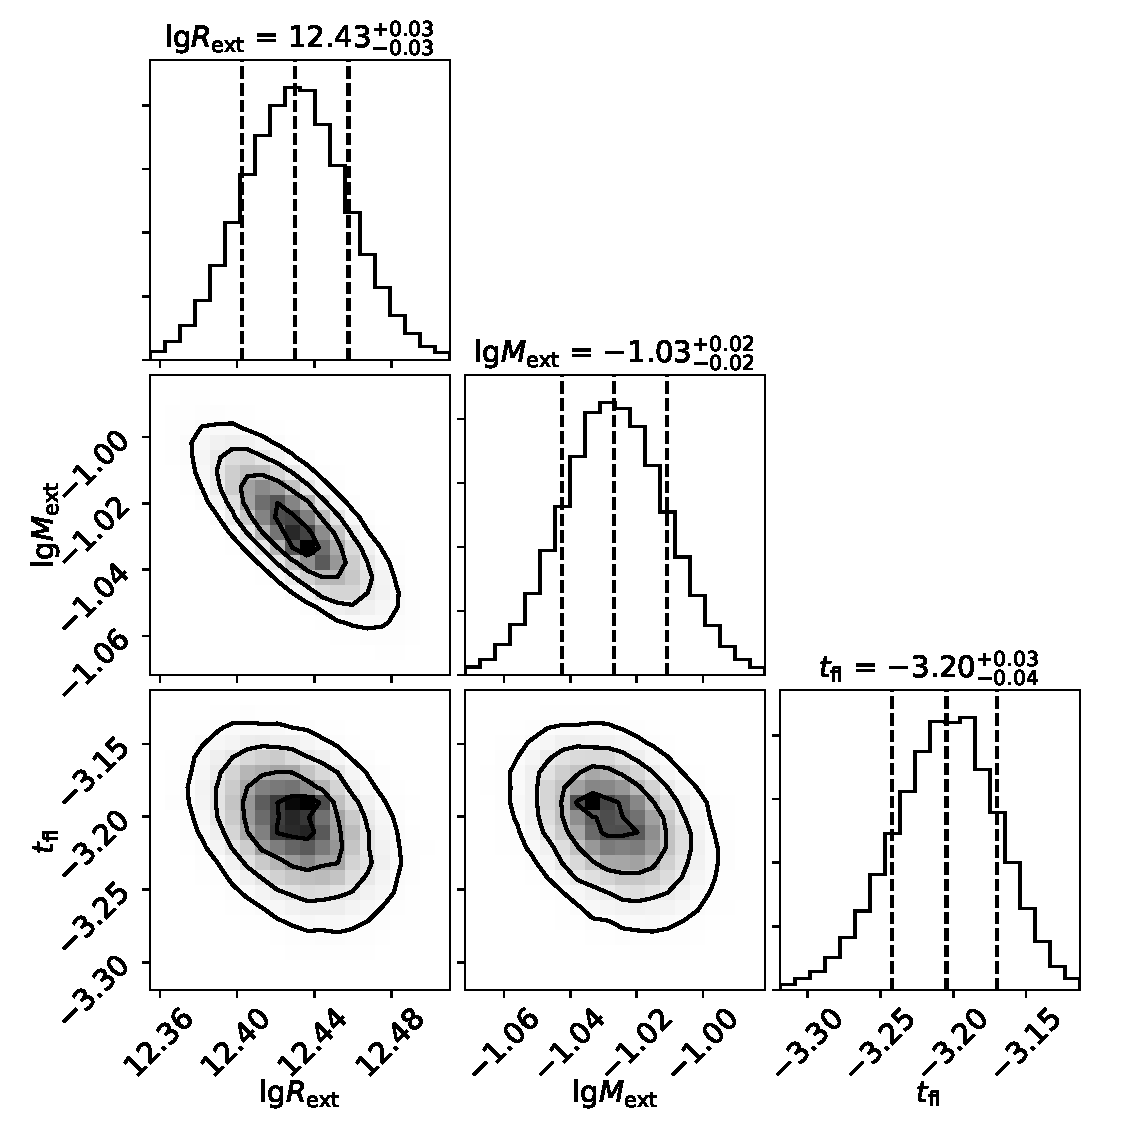
\includegraphics[width=\columnwidth]{figures/corner_P15.pdf}
	\caption{Corner plot showing the posterior constraints on ${\rm lg}R_{\rm ext}$, ${\rm lg}M_{\rm 
			ext}$, and $t_\mathrm{fl}$. Marginalized one-dimensional distributions are shown along the 
		diagonal, along with the median estimate and the 68\% credible region (shown with vertical 
		dashed 
		lines).	\label{fig:pirocorner}}
\end{figure}
To model the early light curve with the P15 model, we fix $\kappa\sim0.2\,{\rm cm^2\, g^{-1}}$ as 
appropriate for a hydrogen-deficient ionized gas, and assign wide flat priors for all model parameters, 
as summarized in Table~\ref{tab:P15priors}. We only include observations up to $\Delta t = 2$\,d in 
the fitting. We found that this particular choice of $\Delta t$ --- 2\,d instead of 1\,d or 3\,d --- in 
general does not affect the final inference for the model parameters. Figure~\ref{fig:pirocorner} shows 
the corner plot of ${\rm lg}R_{\rm ext}$, ${\rm lg}M_{\rm 	ext}$, and $t_\mathrm{fl}$. For clarity, 
$E_{51}$ and $M_{\rm core}$ are excluded as they do not exhibit strong covariance with the 
parameters shown here. We are unable to constrain these two parameters as they are highly 
anti-correlated with each other over a wide range of their priors.

\begin{figure}[htbp!]
	\centering
	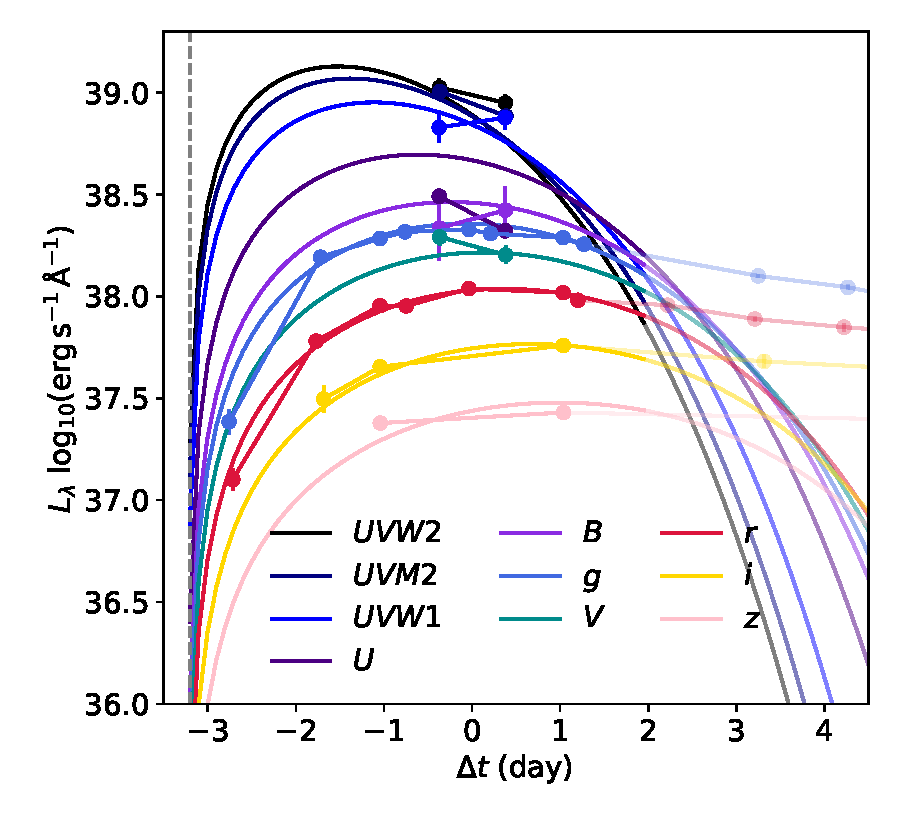
\includegraphics[width=\columnwidth]{figures/P15model.pdf}
	\caption{Cooling emission model fit to the early light curve of AT2019dge. 
		Data excluded from the fitting are shown as transparent circles. 
		The maximum a posteriori model is shown via solid lines.
		The vertical dashed line shows the median 1-D marginalized posterior value of
		$t_{\rm fl}$.
		\label{fig:piromodel}}
\end{figure}

The maximum a posteriori model is visualized by solid lines in Figure~\ref{fig:piromodel} color-coded in 
different filters. Note that the fitting is not perfect at the UV bands since 
the SED is not exactly a blackbody at peak (see Figure~\ref{fig:seds}). The rising part of the model 
does not match to data due to the ignorance of the density structure of the stellar profile. \todo{Ask 
Tony} Nevertheless, the peak of the light curve is well captured by this model.


\section{UV and Optical Spectroscopy} \label{app:spec}
The log of UV and optical spectroscopy is presented in Table \ref{tab:spec}.

\begin{table*}{llcc}
	\caption{Log of AT2019dge spectroscopy. \label{tab:spec}}
	\centering
	\begin{tabular}{llccc}
	\toprule
	Start Time  & Instrument & Expo. Time (s) & Airmass & Resolution\\
	(UTC) & & & & (FWHM $\AA$)\\
	\midrule
	% # DATE-OBS= '2019-04-09T03:30:28.157'             % # UTSTART = '03:30:28.157'
	% # MJD     =         58582.146159
	2019 Apr 09 03:30:28 & LT+SPART  &  500   & 1.800 & 18 \\
	% # DATE-OBS= '2019-04-10T03:06:09.604'
	% # UTSTART = '03:06:09.604'
	% # MJD     =         58583.129278
	2019 Apr 10 03:06:10 & LT+SPART  &  500   & 1.800 & 18 \\
	% LRIS
	2019 Apr 10 14:21:44 & Keck1+LRIS & 300 & 1.169 & 6 \\
	% HST
	2019 Apr 12 05:08:00 & HST+UVIS & 200 & --- & \\
	% DBSP
	2019 Apr 24 11:06:43 & P200+DBSP & 1200 & 1.047 & 3--5\\
	% LRIS
	2019 Jul 04 11:49:18   & Keck1+LRIS & 1740 & 1.421 & 6\\
	% LRIS
	2019 Aug 31 08:04:58   & Keck1+LRIS & 1150 & 1.409 & 6  \\
	% LRIS
	2019 Sep 28 08:14:27   & Keck1+LRIS & 600 & 2.165 & 6\\
	\bottomrule
\end{tabular}
\end{table*}

%The final spectrum taken was a LRIS spectrum from $+111?$\,days which showed narrow nebular 
%emission lines from the host galaxy but no detectable flux from AT2019dge. 
We use line centers of nebular lines to derive the spectroscopic redshift of the host (Table 
\ref{tab:host}). The mean of all centroids gives $z = 0.0213 \pm 0.0001$.

\begin{table}[htbp!]
	\caption{Line fluxes from the host galaxy of AT2019dge extracted from the Keck/LRIS spectrum 
	obtained on Aug xx 2019. }\label{tab:eml_host}
	\centering
	\begin{tabular}{llcc}
		\toprule
		Transition			& $\lambda_{\rm obs}$& $F$	\\
		& (\AA)	& $\left(10^{-16}~{\rm erg\,cm}^{-2}\,{\rm s}^{-1}\right) $ \\
		\midrule
		%{[\ion{O}{2}]}$\lambda\lambda$3726,3729 &$ 3848.17 \pm 0.05	$&$	334.5	\pm	6.23	$\\
		%{[\ion{Ne}{3}]}$\lambda$3869			& $ 3993.50 \pm 0.16	$&$	82.34	\pm	6.18	$\\
		%\ion{He}{1}$\lambda$3889,H-8			& $ 4014.49 \pm 0.16	$&$	29.01	\pm	4.73	$\\
		%{[\ion{Ne}{3}]}$\lambda$3968,H$\epsilon$& $ 4096.66 \pm 0.26	$&$	36.61	\pm	3.98	$\\
		%H$\delta$ 								& $ 4233.87 \pm 0.13	$&$	44.88	\pm	2.59	$\\
		%H$\gamma$								& $ 4480.20 \pm 0.10	$&$	81.95	\pm	3.74	$\\
		%{[\ion{O}{3}]}$\lambda$4364 			& $ 4503.68 \pm 0.10	$&$	15.01	\pm	2.69	$\\
		H$\beta$								& $ 4862.35 \pm 0.21	$ &$	32.45 \pm 2.08		$\\%yes
		%{[\ion{O}{3}]}$\lambda$4960 			& $ 5118.61 \pm 0.04	$&$	352.42	\pm	6.50	$\\
		{[\ion{O}{III}]}$\lambda$5007				& $5007.06 \pm 0.55$ &$67.56 \pm 13.52	$\\%yes
		%\ion{He}{1}$\lambda$5877				& $ 6064.21 \pm 0.20	$&$	27.04	\pm	2.30	$\\
		%\ion{O}{1}$\lambda$6302				& $ 6502.18 \pm 1.08	$&$	6.72	\pm	2.94	$\\
		%{[\ion{N}{2}]}$\lambda$6549				& $ 6758.16 \pm 0.02	$&$	11.15	\pm	6.73	$\\
		H$\alpha$								&$6562.07 	\pm 0.03$   & $115.79 \pm 1.16	$\\%yes
		{[\ion{N}{II}]}$\lambda$6583				& $6582.62 \pm 0.08$ &$	8.89 \pm 0.37	$\\%yes
		%{[\ion{He}{1}]}$\lambda$6678			& $ 6890.29 \pm 0.14	$&$	7.88	\pm	2.19	$\\
		%{[\ion{S}{2}]}$\lambda$6718 			& $ 6931.83 \pm 0.10	$&$	41.76	\pm	2.38	$\\
		%{[\ion{S}{2}]}$\lambda$6732 			& $ 6946.68 \pm 0.10	$&$	28.15	\pm	2.19	$\\
		\bottomrule
	\end{tabular}
	\tablecomments{All measurements are corrected for Galactic reddening.}
\end{table}

\begin{table}
	\centering
	\caption{Photometry of the host galaxy}\label{tab:host_phot}
	\begin{tabular}{ccc}
		\toprule
		Instrument/	    & $\lambda_{\rm eff}$   & Brightness		\\
		Filter          & (\AA)                 & (mag)             \\
		\midrule
		SDSS/$u'$ 		& 3594.9  & $ 19.336	 \pm 0.039$	\\
		SDSS/$g'$ 		& 4640.4  & $ 18.322 \pm 0.009$	\\
		SDSS/$r'$ 		& 6122.3  & $ 17.913	 \pm 0.009 $	 \\
		SDSS/$i'$ 		& 7439.5     &$ 17.745  \pm 0.010$\\
		SDSS/$z'$ 		& 8897.1     &$ 17.580 \pm 0.031$\\
		 WISE/$W1$ 		& 33526.0    &$ 15.938 \pm 0.037$\\
		  WISE/$W2$   & 46028.0    &$ 15.982 \pm  0.082$\\
		\bottomrule
	\end{tabular}
	\tablecomments{All measurements are reported in the AB system and are not corrected for 
	reddening. Reference: SDSS \citep{Alam2015}, AllWISE \citep{Cutri2013}}
\end{table}
% no record in URAT1
% no record in GALEX

\bibliography{at2019dge}{}
\bibliographystyle{aasjournal}

\end{CJK*}


\end{document}